\documentclass[10pt,a4paper]{article}

\usepackage[T1]{fontenc}
\usepackage[utf8]{inputenc}
\usepackage{lmodern}
\usepackage[margin=2.3cm]{geometry}
\usepackage{amsmath,amssymb,amsthm}
\usepackage{graphicx}
\usepackage{booktabs}
\usepackage{array}
\usepackage{adjustbox}
\usepackage{url}
\Urlmuskip=0mu plus 2mu\relax
\usepackage{xcolor}
\usepackage{microtype}
\usepackage{algorithm}
\usepackage{algpseudocode}
\usepackage[hidelinks]{hyperref}
\usepackage{orcidlink}
\usepackage{caption}
\captionsetup{font=small,labelfont=bf}
\setlength{\parskip}{0.4em}
\setlength{\parindent}{0pt}
\setlength{\emergencystretch}{2em}
\newtheorem{proposition}{Proposition}
\newtheorem{conjecture}{Conjecture}
\renewcommand{\algorithmicrequire}{\textbf{Input:}}
\renewcommand{\algorithmicensure}{\textbf{Output:}}

\graphicspath{{../figures/}}
% Numbers measured by data/measure.py (never typed): macros and the result tables.
% The macro file defines a few names twice with the same value (\longALpiMin, \longBLpiMin): read it with \providecommand.
\let\newcommandOriginal\newcommand
\let\newcommand\providecommand
% Generated by data/measure.py from flicker.json. Do not edit.
\newcommand{\engineRelease}{0.02.004}
\newcommand{\parFrames}{13}
\newcommand{\parFrameIters}{10}
\newcommand{\parKimIters}{5}
\newcommand{\parPhaseVel}{0.3}
\newcommand{\parSubsteps}{10}
\newcommand{\claimStepFu}{0.2}
\newcommand{\scopeDefaultFrames}{13}
\newcommand{\scopePhaseVel}{1}
\newcommand{\winMinSeeds}{5}
\newcommand{\winMinDiff}{0.01}
\newcommand{\nSeedsTwo}{6}
\newcommand{\accBTransMed}{0.923}
\newcommand{\accBTransMin}{0.915}
\newcommand{\accBTransMax}{0.932}
\newcommand{\accBTransMean}{0.923}
\newcommand{\accBTransCiLo}{0.916}
\newcommand{\accBTransCiHi}{0.930}
\newcommand{\accBFrameMed}{0.987}
\newcommand{\accBFrameMin}{0.979}
\newcommand{\accBFrameMax}{0.993}
\newcommand{\accBFrameMean}{0.986}
\newcommand{\accBFrameCiLo}{0.980}
\newcommand{\accBFrameCiHi}{0.992}
\newcommand{\accBBlendMed}{0.923}
\newcommand{\accBBlendMin}{0.915}
\newcommand{\accBBlendMax}{0.932}
\newcommand{\accBBlendMean}{0.923}
\newcommand{\accBBlendCiLo}{0.916}
\newcommand{\accBBlendCiHi}{0.930}
\newcommand{\accBStepMed}{0.069}
\newcommand{\accBStepMin}{0.041}
\newcommand{\accBStepMax}{0.077}
\newcommand{\accBStepMean}{0.066}
\newcommand{\accBStepCiLo}{0.052}
\newcommand{\accBStepCiHi}{0.080}
\newcommand{\accBSigmaMed}{0.240}
\newcommand{\accBSigmaMin}{0.106}
\newcommand{\accBSigmaMax}{0.386}
\newcommand{\accBSigmaMean}{0.246}
\newcommand{\accBSigmaCiLo}{0.109}
\newcommand{\accBSigmaCiHi}{0.383}
\newcommand{\accBSecMed}{1.19}
\newcommand{\accBSecMin}{1.01}
\newcommand{\accBSecMax}{1.36}
\newcommand{\accBSecMean}{1.18}
\newcommand{\accBSecCiLo}{1.05}
\newcommand{\accBSecCiHi}{1.31}
\newcommand{\accLpiTransMed}{0.648}
\newcommand{\accLpiTransMin}{0.551}
\newcommand{\accLpiTransMax}{0.709}
\newcommand{\accLpiTransMean}{0.644}
\newcommand{\accLpiTransCiLo}{0.584}
\newcommand{\accLpiTransCiHi}{0.703}
\newcommand{\accLpiFrameMed}{0.652}
\newcommand{\accLpiFrameMin}{0.584}
\newcommand{\accLpiFrameMax}{0.722}
\newcommand{\accLpiFrameMean}{0.656}
\newcommand{\accLpiFrameCiLo}{0.602}
\newcommand{\accLpiFrameCiHi}{0.711}
\newcommand{\accLpiBlendMed}{0.648}
\newcommand{\accLpiBlendMin}{0.551}
\newcommand{\accLpiBlendMax}{0.709}
\newcommand{\accLpiBlendMean}{0.644}
\newcommand{\accLpiBlendCiLo}{0.584}
\newcommand{\accLpiBlendCiHi}{0.703}
\newcommand{\accLpiStepMed}{0.409}
\newcommand{\accLpiStepMin}{0.300}
\newcommand{\accLpiStepMax}{0.476}
\newcommand{\accLpiStepMean}{0.392}
\newcommand{\accLpiStepCiLo}{0.317}
\newcommand{\accLpiStepCiHi}{0.467}
\newcommand{\accLpiSigmaMed}{23.497}
\newcommand{\accLpiSigmaMin}{19.157}
\newcommand{\accLpiSigmaMax}{27.017}
\newcommand{\accLpiSigmaMean}{23.000}
\newcommand{\accLpiSigmaCiLo}{19.926}
\newcommand{\accLpiSigmaCiHi}{26.073}
\newcommand{\accLpiSecMed}{1.63}
\newcommand{\accLpiSecMin}{1.60}
\newcommand{\accLpiSecMax}{2.20}
\newcommand{\accLpiSecMean}{1.73}
\newcommand{\accLpiSecCiLo}{1.48}
\newcommand{\accLpiSecCiHi}{1.97}
\newcommand{\accKimFiveTransMed}{0.953}
\newcommand{\accKimFiveTransMin}{0.918}
\newcommand{\accKimFiveTransMax}{0.965}
\newcommand{\accKimFiveTransMean}{0.948}
\newcommand{\accKimFiveTransCiLo}{0.929}
\newcommand{\accKimFiveTransCiHi}{0.966}
\newcommand{\accKimFiveFrameMed}{0.973}
\newcommand{\accKimFiveFrameMin}{0.944}
\newcommand{\accKimFiveFrameMax}{0.984}
\newcommand{\accKimFiveFrameMean}{0.967}
\newcommand{\accKimFiveFrameCiLo}{0.949}
\newcommand{\accKimFiveFrameCiHi}{0.984}
\newcommand{\accKimFiveBlendMed}{0.953}
\newcommand{\accKimFiveBlendMin}{0.918}
\newcommand{\accKimFiveBlendMax}{0.965}
\newcommand{\accKimFiveBlendMean}{0.948}
\newcommand{\accKimFiveBlendCiLo}{0.929}
\newcommand{\accKimFiveBlendCiHi}{0.966}
\newcommand{\accKimFiveStepMed}{0.302}
\newcommand{\accKimFiveStepMin}{0.114}
\newcommand{\accKimFiveStepMax}{0.408}
\newcommand{\accKimFiveStepMean}{0.279}
\newcommand{\accKimFiveStepCiLo}{0.169}
\newcommand{\accKimFiveStepCiHi}{0.388}
\newcommand{\accKimFiveSigmaMed}{2.228}
\newcommand{\accKimFiveSigmaMin}{0.719}
\newcommand{\accKimFiveSigmaMax}{2.876}
\newcommand{\accKimFiveSigmaMean}{2.041}
\newcommand{\accKimFiveSigmaCiLo}{1.214}
\newcommand{\accKimFiveSigmaCiHi}{2.868}
\newcommand{\accKimFiveSecMed}{0.59}
\newcommand{\accKimFiveSecMin}{0.51}
\newcommand{\accKimFiveSecMax}{0.67}
\newcommand{\accKimFiveSecMean}{0.60}
\newcommand{\accKimFiveSecCiLo}{0.54}
\newcommand{\accKimFiveSecCiHi}{0.66}
\newcommand{\accKimTenTransMed}{0.926}
\newcommand{\accKimTenTransMin}{0.880}
\newcommand{\accKimTenTransMax}{0.966}
\newcommand{\accKimTenTransMean}{0.925}
\newcommand{\accKimTenTransCiLo}{0.890}
\newcommand{\accKimTenTransCiHi}{0.961}
\newcommand{\accKimTenFrameMed}{0.981}
\newcommand{\accKimTenFrameMin}{0.955}
\newcommand{\accKimTenFrameMax}{0.986}
\newcommand{\accKimTenFrameMean}{0.975}
\newcommand{\accKimTenFrameCiLo}{0.961}
\newcommand{\accKimTenFrameCiHi}{0.989}
\newcommand{\accKimTenBlendMed}{0.926}
\newcommand{\accKimTenBlendMin}{0.880}
\newcommand{\accKimTenBlendMax}{0.966}
\newcommand{\accKimTenBlendMean}{0.925}
\newcommand{\accKimTenBlendCiLo}{0.890}
\newcommand{\accKimTenBlendCiHi}{0.961}
\newcommand{\accKimTenStepMed}{0.499}
\newcommand{\accKimTenStepMin}{0.145}
\newcommand{\accKimTenStepMax}{0.619}
\newcommand{\accKimTenStepMean}{0.427}
\newcommand{\accKimTenStepCiLo}{0.225}
\newcommand{\accKimTenStepCiHi}{0.630}
\newcommand{\accKimTenSigmaMed}{1.287}
\newcommand{\accKimTenSigmaMin}{0.719}
\newcommand{\accKimTenSigmaMax}{1.844}
\newcommand{\accKimTenSigmaMean}{1.242}
\newcommand{\accKimTenSigmaCiLo}{0.785}
\newcommand{\accKimTenSigmaCiHi}{1.698}
\newcommand{\accKimTenSecMed}{0.94}
\newcommand{\accKimTenSecMin}{0.86}
\newcommand{\accKimTenSecMax}{1.05}
\newcommand{\accKimTenSecMean}{0.95}
\newcommand{\accKimTenSecCiLo}{0.88}
\newcommand{\accKimTenSecCiHi}{1.02}
\newcommand{\bTwoMin}{0.915}
\newcommand{\bTwoMed}{0.923}
\newcommand{\bTwoMax}{0.932}
\newcommand{\lpiMin}{0.551}
\newcommand{\lpiMed}{0.648}
\newcommand{\lpiMax}{0.709}
\newcommand{\bTwoSigmaFrame}{0.39}
\newcommand{\lpiSigmaFrameMin}{19}
\newcommand{\lpiSigmaFrameMax}{27}
\newcommand{\bTwoSigmaFrameMed}{0.24}
\newcommand{\lpiSigmaFrameMed}{23.5}
\newcommand{\sigmaFrameFactorLo}{50}
\newcommand{\sigmaFrameFactorHi}{70}
\newcommand{\bTwoMean}{0.923}
\newcommand{\bTwoSd}{0.007}
\newcommand{\bTwoCiLo}{0.916}
\newcommand{\bTwoCiHi}{0.930}
\newcommand{\lpiMean}{0.644}
\newcommand{\lpiSd}{0.057}
\newcommand{\lpiCiLo}{0.584}
\newcommand{\lpiCiHi}{0.703}
\newcommand{\diffTwoMean}{0.279}
\newcommand{\diffTwoCiLo}{0.218}
\newcommand{\diffTwoCiHi}{0.340}
\newcommand{\bTwoMedSeven}{0.754}
\newcommand{\bTwoMinSeven}{0.735}
\newcommand{\lpiMedSeven}{0.621}
\newcommand{\lpiMaxSeven}{0.666}
\newcommand{\bTwoMedTwentyFive}{0.973}
\newcommand{\bTwoMinTwentyFive}{0.963}
\newcommand{\lpiMedTwentyFive}{0.648}
\newcommand{\lpiMaxTwentyFive}{0.722}
\newcommand{\readThirteenLpiDip}{proposed}
\newcommand{\readThirteenLpiDipN}{6 and 6}
\newcommand{\readThirteenLpiSigma}{proposed}
\newcommand{\readThirteenLpiSigmaN}{6 and 6}
\newcommand{\readThirteenKimFiveDip}{published}
\newcommand{\readThirteenKimFiveDipN}{6 and 6}
\newcommand{\readThirteenKimFiveSigma}{proposed}
\newcommand{\readThirteenKimFiveSigmaN}{6 and 6}
\newcommand{\readThirteenKimTenDip}{tie}
\newcommand{\readThirteenKimTenDipN}{6 and 6}
\newcommand{\readThirteenKimTenSigma}{proposed}
\newcommand{\readThirteenKimTenSigmaN}{6 and 6}
\newcommand{\readSevenLpiDip}{proposed}
\newcommand{\readSevenLpiDipN}{6 and 6}
\newcommand{\readSevenLpiSigma}{proposed}
\newcommand{\readSevenLpiSigmaN}{6 and 6}
\newcommand{\readSevenKimFiveDip}{published}
\newcommand{\readSevenKimFiveDipN}{6 and 6}
\newcommand{\readSevenKimFiveSigma}{proposed}
\newcommand{\readSevenKimFiveSigmaN}{6 and 6}
\newcommand{\readSevenKimTenDip}{published}
\newcommand{\readSevenKimTenDipN}{6 and 6}
\newcommand{\readSevenKimTenSigma}{proposed}
\newcommand{\readSevenKimTenSigmaN}{6 and 6}
\newcommand{\readTwentyFiveLpiDip}{proposed}
\newcommand{\readTwentyFiveLpiDipN}{6 and 6}
\newcommand{\readTwentyFiveLpiSigma}{proposed}
\newcommand{\readTwentyFiveLpiSigmaN}{6 and 6}
\newcommand{\readTwentyFiveKimFiveDip}{tie}
\newcommand{\readTwentyFiveKimFiveDipN}{6 and 6}
\newcommand{\readTwentyFiveKimFiveSigma}{proposed}
\newcommand{\readTwentyFiveKimFiveSigmaN}{6 and 6}
\newcommand{\readTwentyFiveKimTenDip}{tie}
\newcommand{\readTwentyFiveKimTenDipN}{6 and 6}
\newcommand{\readTwentyFiveKimTenSigma}{proposed}
\newcommand{\readTwentyFiveKimTenSigmaN}{6 and 6}
\newcommand{\accFu}{2.00}
\newcommand{\accPeakStep}{0.31}
\newcommand{\accFramesForMove}{20}
\newcommand{\accFramesBoundMinimum}{20}
\newcommand{\deltaNine}{0.356}
\newcommand{\sincAcc}{0.922}
\newcommand{\sincClaim}{0.968}
\newcommand{\longABins}{12}
\newcommand{\longAFu}{6}
\newcommand{\longAFrames}{58}
\newcommand{\longAMed}{0.933}
\newcommand{\longAMet}{6}
\newcommand{\longALow}{0.023}
\newcommand{\longAPeakStep}{0.197}
\newcommand{\longABound}{58}
\newcommand{\longALpiMin}{0.568}
\newcommand{\longALpiMax}{0.756}
\newcommand{\longABLeadsLpi}{7}
\newcommand{\longAKimFiveMin}{0.927}
\newcommand{\longAKimFiveMax}{0.976}
\newcommand{\longABLeadsKimFive}{2}
\newcommand{\longAKimTenMin}{0.912}
\newcommand{\longAKimTenMax}{0.978}
\newcommand{\longABLeadsKimTen}{2}
\newcommand{\longABLeads}{7}
\newcommand{\longALpiMin}{0.568}
\newcommand{\longALpiMax}{0.756}
\newcommand{\longAReadLpi}{proposed}
\newcommand{\longAReadKimFive}{tie}
\newcommand{\longAReadKimTen}{tie}
\newcommand{\longBBins}{20}
\newcommand{\longBFu}{10}
\newcommand{\longBFrames}{95}
\newcommand{\longBMed}{0.936}
\newcommand{\longBMet}{6}
\newcommand{\longBLow}{0.584}
\newcommand{\longBPeakStep}{0.199}
\newcommand{\longBBound}{95}
\newcommand{\longBLpiMin}{0.581}
\newcommand{\longBLpiMax}{0.701}
\newcommand{\longBBLeadsLpi}{7}
\newcommand{\longBKimFiveMin}{0.928}
\newcommand{\longBKimFiveMax}{0.976}
\newcommand{\longBBLeadsKimFive}{1}
\newcommand{\longBKimTenMin}{0.908}
\newcommand{\longBKimTenMax}{0.979}
\newcommand{\longBBLeadsKimTen}{2}
\newcommand{\longBBLeads}{7}
\newcommand{\longBLpiMin}{0.581}
\newcommand{\longBLpiMax}{0.701}
\newcommand{\longBReadLpi}{proposed}
\newcommand{\longBReadKimFive}{published}
\newcommand{\longBReadKimTen}{tie}
\newcommand{\longSeeds}{8}
\newcommand{\longAPeak}{0.197}
\newcommand{\longBPeak}{0.199}
\newcommand{\longFailList}{0.768 and 0.023 at 12 bins; 0.584 and 0.847 at 20 bins}
\newcommand{\longTwiceList}{0.757 and 0.000 at 12 bins; 0.558 and 0.840 at 20 bins}
\newcommand{\longDefaultMax}{0.528}
\newcommand{\cTenMoving}{16}
\newcommand{\cTenTraps}{36}
\newcommand{\cTenFu}{14.5}
\newcommand{\cTenFrames}{137}
\newcommand{\cTenEqual}{25}
\newcommand{\cTenPeakEqual}{1.13}
\newcommand{\cTenPeak}{0.200}
\newcommand{\cTenHeld}{0.232}
\newcommand{\cTenSeeds}{6}
\newcommand{\cTenLpiLeads}{4}
\newcommand{\cTenBEqualMax}{0.412}
\newcommand{\cTenLEqualMin}{0.024}
\newcommand{\cTenLEqualMax}{0.616}
\newcommand{\cTenMet}{6}
\newcommand{\cTenMetMin}{0.909}
\newcommand{\cTenMetMax}{0.917}
\newcommand{\cTenMetMed}{0.914}
\newcommand{\cTenLowest}{0.909}
\newcommand{\cTenLpiMin}{0.044}
\newcommand{\cTenLpiMax}{0.738}
\newcommand{\cTenBLeads}{6}
\newcommand{\cTenKimFiveMin}{0.922}
\newcommand{\cTenKimFiveMax}{0.956}
\newcommand{\cTenBLeadsKimFive}{0}
\newcommand{\cTenKimTenMin}{0.846}
\newcommand{\cTenKimTenMax}{0.936}
\newcommand{\cTenBLeadsKimTen}{2}
\newcommand{\cTenFailList}{none}
\newcommand{\cTenReadLpi}{proposed}
\newcommand{\cTenReadLpiN}{6 and 6}
\newcommand{\cTenReadKimFive}{published}
\newcommand{\cTenReadKimFiveN}{6 and 6}
\newcommand{\cTenReadKimTen}{tie}
\newcommand{\cTenReadKimTenN}{6 and 6}
\newcommand{\phaseStepBMax}{0.077}
\newcommand{\phaseStepKimFiveMax}{0.408}
\newcommand{\phaseStepKimTenMax}{0.619}
\newcommand{\phaseStepLpiMax}{0.476}
\newcommand{\ablTFullMed}{0.923}
\newcommand{\ablTFullMin}{0.915}
\newcommand{\ablTFullMax}{0.932}
\newcommand{\ablTFullMean}{0.923}
\newcommand{\ablTFullSd}{0.007}
\newcommand{\ablTFullSig}{0.24}
\newcommand{\ablTFullStep}{0.069}
\newcommand{\ablTNoLockMed}{0.905}
\newcommand{\ablTNoLockMin}{0.776}
\newcommand{\ablTNoLockMax}{0.924}
\newcommand{\ablTNoLockMean}{0.884}
\newcommand{\ablTNoLockSd}{0.055}
\newcommand{\ablTNoLockSig}{2.45}
\newcommand{\ablTNoLockStep}{0.455}
\newcommand{\ablTNoOptMed}{0.803}
\newcommand{\ablTNoOptMin}{0.724}
\newcommand{\ablTNoOptMax}{0.830}
\newcommand{\ablTNoOptMean}{0.789}
\newcommand{\ablTNoOptSd}{0.038}
\newcommand{\ablTNoOptSig}{17.67}
\newcommand{\ablTNoOptStep}{0.064}
\newcommand{\ablTItersOneMed}{0.744}
\newcommand{\ablTItersOneMin}{0.676}
\newcommand{\ablTItersOneMax}{0.823}
\newcommand{\ablTItersOneMean}{0.747}
\newcommand{\ablTItersOneSd}{0.069}
\newcommand{\ablTItersOneSig}{18.62}
\newcommand{\ablTItersOneStep}{0.063}
\newcommand{\ablTItersThreeMed}{0.916}
\newcommand{\ablTItersThreeMin}{0.905}
\newcommand{\ablTItersThreeMax}{0.933}
\newcommand{\ablTItersThreeMean}{0.918}
\newcommand{\ablTItersThreeSd}{0.010}
\newcommand{\ablTItersThreeSig}{3.50}
\newcommand{\ablTItersThreeStep}{0.066}
\newcommand{\ablTLinearMed}{0.968}
\newcommand{\ablTLinearMin}{0.959}
\newcommand{\ablTLinearMax}{0.974}
\newcommand{\ablTLinearMean}{0.967}
\newcommand{\ablTLinearSd}{0.006}
\newcommand{\ablTLinearSig}{0.21}
\newcommand{\ablTLinearStep}{0.041}
\newcommand{\ablTN}{6}
\newcommand{\ablTCheck}{0.0e+00}
\newcommand{\ablSeconds}{1}
\newcommand{\mainMinutes}{2}

\let\newcommand\newcommandOriginal
% Quantities computed from those macros only (TeX arithmetic), so that no derived number is typed either.
\newcommand{\stepRatio}{\fpeval{round(\accKimFiveStepMax/\accBStepMax,1)}}
\newcommand{\stepRatioTen}{\fpeval{round(\accKimTenStepMax/\accBStepMax,1)}}
\newcommand{\stepRatioLpi}{\fpeval{round(\accLpiStepMax/\accBStepMax,1)}}
\newcommand{\sigmaRatio}{\fpeval{round(\accKimFiveSigmaMed/\accBSigmaMed,1)}}
\newcommand{\dipGap}{\fpeval{round(\accKimFiveTransMean-\accBTransMean,3)}}
\newcommand{\secRatio}{\fpeval{round(\accBSecMean/\accKimFiveSecMean,1)}}
\newcommand{\lockStepRatio}{\fpeval{round(\ablTNoLockStep/\ablTFullStep,1)}}
\newcommand{\linearGap}{\fpeval{round(\ablTLinearMean-\accKimFiveTransMean,3)}}
% Design constants of the simulated setup (data/measure.py, make_setup): not results.
\newcommand{\setupLambda}{850}
\newcommand{\setupFocal}{250}
\newcommand{\setupPitch}{12.5}
\newcommand{\setupNpix}{256}
\newcommand{\setupPad}{2}
\newcommand{\setupNa}{0.5}
\newcommand{\setupCold}{30}

% Page-1 header block (conventions/manuscript-header-standard.md). The four document macros are set by the
% publishing tool when the version DOI is reserved.
\newcommand{\doctype}{Preprint}
\newcommand{\docversion}{v0.02}
\newcommand{\docdate}{2026-11-20}
\newcommand{\versiondoi}{10.5281/zenodo.24385662}
\newcommand{\conceptdoi}{10.5281/zenodo.24267369}
\newcommand{\docrepo}{github.com/fsantibanezleal/CEFOP\_DinHot}
\newcommand{\headerblock}{%
\begin{center}
\fbox{\parbox{0.94\textwidth}{\small\raggedright
\textbf{\doctype} \quad$\cdot$\quad \docversion, \docdate \quad$\cdot$\quad Licence CC BY 4.0\\[2pt]
CAOS open-research programme \quad$\cdot$\quad CEFOP\_DinHot, holographic optical trap studio\\[2pt]
Version DOI \href{https://doi.org/\versiondoi}{\texttt{\versiondoi}} \quad$\cdot$\quad
concept DOI (always latest) \href{https://doi.org/\conceptdoi}{\texttt{\conceptdoi}}\\[2pt]
Not peer reviewed. Source code, data and computational records: \href{https://\docrepo}{\texttt{\docrepo}}
}}
\end{center}
\vspace{4pt}}

\begin{document}

\title{Flicker-Bounded Phase-Continuous Hologram Sequences for Moving Optical Traps: Smaller Phase Steps than Per-Frame Gerchberg-Saxton, a Higher Transient Minimum with a Linear Time Profile on the Short Move and a Lower One with the Minimal-Jerk Profile}
\author{Felipe Santib\'a\~nez-Leal~\orcidlink{0000-0002-0150-3246}\\
\small CAOS open-research programme, Santiago, Chile\\
\small \texttt{fsantibanez@gmail.com}}
\date{}
\maketitle
\vspace{-1.2em}
\headerblock

\begin{abstract}
Atoms in optical tweezer arrays are rearranged by moving the traps with a sequence of holograms on a spatial light modulator. Published sequences either compute every frame by Gerchberg--Saxton iterations started from the previous frame's phase (phase induction), or interpolate the trap phases linearly between two endpoint holograms. We propose a flicker-bounded phase-continuous sequence: every frame is a weighted Gerchberg--Saxton step whose trap phases are locked to a smooth prescribed trajectory, and a frame-count equation bounds the shift of the pattern between frames. On a $4\times4$ lattice with eight traps moved over \parFrames{} frames and \nSeedsTwo{} seeds, the lowest transient intensity of a moving trap is \accBTransMean{} of its mean with the default minimal-jerk time profile, against \accLpiTransMean{} for linear phase interpolation and \accKimFiveTransMean{} for the per-frame sequence with phase induction, which the benchmark rule reads as better on the dip. With the linear profile that the baselines use, a comparison added after the results and run on this move only, the sequence reaches \ablTLinearMean{} and the rule reads it as better than every baseline. Its largest phase step stays below that of the per-frame sequence in both profiles (\accBStepMax{} against \accKimFiveStepMax{} rad at the default profile). On a sort of 36 traps the per-frame sequence is higher on every seed, and on long lattice moves with the frames of the bound the default sequence reaches 0.9 on \longAMet{} of \longSeeds{} seeds and the per-frame sequence on all. All results are simulated on a scalar model.
\end{abstract}

\noindent\textbf{Keywords:} holographic optical tweezers, atom rearrangement, Gerchberg--Saxton algorithm, phase continuity, linear phase interpolation, spatial light modulator.

\section{Introduction}\label{sec:intro}

Neutral-atom quantum processors and simulators start every experimental cycle from a stochastically loaded array of optical tweezers, in which about half of the sites hold an atom. The atoms are sorted into a defect-free target pattern before the computation or the simulation begins. Defect-free arrays of hundreds of atoms support the programmable simulators and the logical-qubit processors that now operate~\cite{ebadi,bluvstein}, arrays of about 6100 atoms have been assembled~\cite{manetsch}, and an architecture that keeps more than 3000 atoms for hours reloads the array continuously~\cite{chiu}. The time and the loss probability of the sorting step enter the yield of every cycle, so the way the traps are moved is a design question of the experiment and not a detail of its control software.

Two families of machines sort atoms. Acousto-optic deflectors move one row or one column of traps at a time, so that the number of moves grows with the size of the array~\cite{endres,barredo}. A spatial light modulator (SLM) displays a hologram that forms all the traps, and a sequence of holograms moves every trap in parallel; the number of moves does not depend on the number of atoms. The SLM route was demonstrated with traps whose movement was designed analytically as a linear combination of linear phases, which is flicker-free by construction for a single trap per sub-plane of the SLM~\cite{kim2016}. For arbitrary geometries the holograms are computed by iterative algorithms of the Gerchberg--Saxton family. Kim, Kim, Lee and Ahn computed every frame of a rearrangement movie by a weighted Gerchberg--Saxton iteration that starts from the phase of the previous frame, which they call phase induction, and which keeps the phases of the traps continuous from frame to frame~\cite{kimoe}. Knottnerus and co-workers instead compute two endpoint holograms and interpolate the position, the amplitude and the optical phase of every trap linearly between them, which they call linear phase interpolation~\cite{lpi}.

The two published sequences leave a different part of the problem open. Linear phase interpolation never optimizes the intermediate frames, so the intensities of the traps in those frames are uneven, and the transient between two frames can dip. Per-frame Gerchberg--Saxton optimizes every frame, and the induction makes the phase of each trap start from its value in the previous frame, but nothing prescribes where the phase of a trap goes: the optimization is free to move it, and the only statement about its size is that the similarity of successive phases, a change small compared with one radian, is empirically guaranteed by the induction~\cite{kimoe}. For the number of frames, Kim et al.\ give a rule (enough frames that the step of a trap is at most the waist of the trap) and an empirical Gaussian fit of the transient minimum against the step; neither published method gives a closed form that turns a stated transient level into a frame count.

We propose the flicker-bounded phase-continuous sequence. Each frame is a weighted Gerchberg--Saxton step whose trap phases are locked to a smooth prescribed trajectory, started from the hologram and the weights of the previous frame, and the number of frames follows from a closed form for the intensity of a trap that is read half way between two frames. It would be wrong to claim that no published work optimizes the intermediate frames of a trap trajectory: Kim et al.~\cite{kimoe} compute every frame. The claim made here is narrower and is tested against that method: the phase trajectory of the traps is prescribed and locked, and the number of frames has a derived bound.

The contributions are the following.
\begin{enumerate}
\item The sequence itself: a hard lock of the trap phases to a minimal-jerk trajectory inside a warm-started weighted iteration, with the frame-count equation that bounds the pattern shift between frames (Section~\ref{sec:flicker-method}).
\item The theory that explains the bound: a closed form for the intensity of a shifted pattern between two frames, a bound on how far the lock lets the achieved trap phase move, and the conditions under which the closed form is only an upper estimate (Section~\ref{sec:theory}).
\item A controlled comparison with both published sequences, linear phase interpolation and per-frame Gerchberg--Saxton with phase induction at 5 and at 10 iterations per frame, run by the same code on the same trajectories, on the acceptance task, on long lattice moves and on the sort of a $6\times6$ array (Sections~\ref{sec:design} and~\ref{sec:results}).
\item An ablation that separates the lock, the per-frame optimization, the iteration count and the time profile (Section~\ref{sec:ablation}).
\item A statement of the trade that the measurements support, including the measures on which the published per-frame method is better (Section~\ref{sec:discussion}).
\end{enumerate}

The main result is a trade that depends on the time profile of the trap positions. With its default minimal-jerk profile and \parFrames{} frames the sequence keeps the lowest moving trap at \accBTransMean{} of its mean against \accLpiTransMean{} for linear phase interpolation, but the per-frame Gerchberg--Saxton sequence of Kim et al.\ keeps it at \accKimFiveTransMean{}. With the constant-velocity profile that the baselines use, in a comparison added after the results (Section~\ref{sec:design}), the same sequence reaches \ablTLinearMean{} and is read as better than all three baselines on the dip. In both profiles it has the smaller largest phase step, \stepRatio{} times smaller than that of the per-frame method at the default profile, and a per-frame intensity spread that is lower by a factor of \sigmaRatio{}. What it costs is a time per sequence of \secRatio{} times that of the per-frame method at its own iteration count, and, with the default profile on the longest moves, seeds on which the prescribed phase path cannot be followed and a sort on which the per-frame method is higher on every seed.

Section~\ref{sec:related} places the sequence among the published methods and Section~\ref{sec:problem} fixes the model, the blend of two frames and the metrics. Section~\ref{sec:flicker-method} defines the sequence with its algorithm, parameters and cost, and Section~\ref{sec:theory} gives the propositions. Sections~\ref{sec:design} to~\ref{sec:ablation} give the experiments, Section~\ref{sec:discussion} reads them against the problem, and Section~\ref{sec:limits} states what the measurements do not show.

\section{Related work}\label{sec:related}

The sequence of this paper touches four bodies of work: the machines that sort atoms and the way their traps are moved, the two published sequences of SLM holograms for rearrangement, the static solvers that compute any single frame, and the corrections for the device that displays the frames. Each is characterised below by what it assumes, what it gives and where it stops short for a moving trap.

\subsection{Machines that sort atoms and the assignment of atoms to sites}

Atom sorting was first demonstrated with moving tweezers steered by acousto-optic deflectors. Endres et al.\ assembled defect-free one-dimensional arrays of more than 50 atoms in less than 400 ms with real-time control of 100 tweezers, replacing lost atoms with surplus ones~\cite{endres}. Barredo et al.\ prepared fully loaded two-dimensional arrays of about 50 microtraps in arbitrary geometries, starting from half-filled matrices and moving atoms with a rapid sequence of moves that depends on the initial distribution~\cite{barredo}. Both machines move one trap, or one row, at a time, so that the number of moves grows with the number of atoms to be placed. Lee, Kim and Ahn framed the choice of which atom goes to which site as a combinatorial assignment problem and solved it with the Hungarian algorithm, which is fast and gives the optimal pairing for the cost they choose~\cite{lee2017}; the sequence of this paper takes that assignment as given and shares it with every baseline. Large processors keep the SLM static and add deflectors for the fast moves of a few atoms: a coherent 3000-qubit system reloads atoms continuously on top of a static array~\cite{chiu}, and a logical processor with up to 280 physical qubits moves atoms between the zones of a reconfigurable array~\cite{bluvstein}. These machines state the time and loss limits of a move but do not specify the hologram sequence; the sequences below do.

\subsection{Analytic moves by linear phases}

Kim et al.\ moved single atoms with holographic microtraps controlled by a liquid-crystal SLM and devised an analytical design of a flicker-free movement~\cite{kim2016}. In their construction a trap is a linear phase over a sub-plane of the SLM, and the linear combination $\alpha k_1x+(1-\alpha)k_2x$ of two linear phases is again a linear phase, so that the focal point sweeps smoothly between the two positions; to obtain several traps the modulation plane is divided into sub-planes, each with its own linear phase. They reported real-time transport with feedback control and a success rate of 99 percent for translations up to 10 micrometres. The construction is flicker-free by design, but it divides the SLM among the traps, so that every trap is formed by a fraction of the pixels, and the pattern is not the interference of all the traps over the whole aperture that a Gerchberg--Saxton hologram forms. It does not apply to a hologram computed by iteration, which is the case of this paper.

\subsection{Per-frame Gerchberg--Saxton with phase induction}

Kim, Kim, Lee and Ahn computed every hologram of a rearrangement movie with a modified Gerchberg--Saxton algorithm that adds zero-padding expansion of the hologram, weighted iteration feedback for reduced crosstalk, and phase induction for successive phase continuity~\cite{kimoe}. With it they formed defect-free two-dimensional atom arrays of various geometries with a loading probability of 0.98 for up to about 30 atoms, and they report a computational scalability up to order $10^3$. In the paper, each frame is generated by a fixed number of iterations toward the trap positions of that frame; the weighted feedback rescales the target by the realised amplitude at the traps relative to its mean; and the induction takes the phase of the previous frame as the initial phase of the next frame, with a condition that the change of phase between frames is small compared with one radian. The numerical experiment of their Fig.~3 uses 5 iterations per frame. They also describe a phase-change reduction (their Eqs.~4 and~5) that they did not use in their experiments. This is the published method against which the sequence is measured; we call it per-frame Gerchberg--Saxton with phase induction and run it as the paper describes it, with the weighted Gerchberg--Saxton rule of the engine (Section~\ref{sec:design}).

The induction differs from a prescription. It chooses the starting point of the iteration, so the phases of the traps start continuous; the optimization is then free to move them, and the phase of each trap at the end of a frame is whatever the iteration reaches. The passages of the paper that define the method, the induction and the weighted feedback, contain no equation that fixes where the trap phases should go along the trajectory and none that gives a number of frames for a stated intensity floor; the frame count is a parameter of the experiment.

\subsection{Linear phase interpolation}

Knottnerus et al.\ computed two endpoint holograms by weighted Gerchberg--Saxton, read the position, the amplitude and the optical phase of every tweezer from them by a Fourier transform, interpolated the three linearly, and inverted the transform at every step~\cite{lpi}. They report cycles of computation and display of 2.736 ms on commercial hardware, a success probability of 0.996 per rearrangement cycle, and, on a separate test setup with an 11 kHz camera, that a single spot made by holograms of the weighted algorithm nearly vanished several times during a move, while the interpolated spot with identical initial and final phase stayed above 70 percent. They also measured the survival of atoms against a phase slip per hologram: slips of up to several tenths of $\pi$ per step did not drastically change the survival, and slips around $\pi$ lost atoms. Their description of earlier work is that all holograms for rearrangement were calculated with the weighted algorithm, which leaves the phases of the tweezers free so that they can jump from hologram to hologram~\cite{lpi}. That statement describes holograms computed independently; the induction of Kim et al.\ is the published remedy for exactly that jump, and the measurement of this paper therefore compares the sequence with linear phase interpolation and with the induced sequence, not with independent frames. Linear phase interpolation does not optimize its intermediate frames: a frame is the inverse transform of interpolated spots, so the intensities of its traps are uneven.

\subsection{Static solvers that compute a single frame}

Every frame of a sequence is a hologram for a set of point traps, and the solvers for that problem are the building blocks. Di Leonardo et al.\ proposed an iterative algorithm for optimal holograms of arbitrary three-dimensional arrangements of traps and showed that the algorithms lead to a phase distribution that maximizes a performance quantifier expressed through the trap intensities, with a weighted form of unprecedented efficiency and uniformity~\cite{dileonardo}. Bianchi and Di Leonardo moved the weighted iteration to a graphics processor for real-time use~\cite{bianchi}. Polin et al.\ optimized holographic traps by direct search and introduced a statistical measure of their performance~\cite{polin}. For arrays of about a thousand foci, Kim et al.\ identified and removed an undesired phase rotation in the iterative Fourier transform algorithm and reached an intensity uniformity above 98 percent after three adaptive correction steps~\cite{kimol}; solvers of this family compute the arrays of a programmable simulator of 256 atoms~\cite{ebadi} and the array of about 6100 atoms~\cite{manetsch}. A different paper of the same year with a similar first-author name, in a different journal, is the source of this phase-fixed rule, and it is cited under its own key; it is not the rearrangement paper of Kim et al.\ discussed above. The frame update of the sequence proposed here is that phase-fixed rule with the phases locked.

\subsection{Camera feedback and the device}

Feedback closes the gap between the model and the instrument. Nogrette et al.\ held single atoms in arrays of up to 100 traps in arbitrary geometries~\cite{nogrette}, and Chew et al.\ reached a relative standard deviation of the tweezer intensity of 0.3 percent with a series of optimization methods driven by precise measurements~\cite{chew}; a feedback algorithm for multi-spot tweezers reports non-uniformity below 1.1 percent for more than a thousand traps~\cite{wang}. The device adds effects that the solvers do not model. A twisted-nematic liquid-crystal display shows fluctuations of its phase modulation on the order of milliseconds~\cite{lizana}, which is the time scale of a frame. Pixel crosstalk is modelled inside conjugate-gradient minimization~\cite{schroff} and inside a modified weighted algorithm~\cite{persson}. None of these treats the frames of a moving-trap sequence; this paper models the transition between two frames as a blend of their fields and does not model the temporal response of the device. The device matters for a moving trap in a way that it does not for a static one: a static array is corrected once by feedback, whereas a sequence is displayed frame after frame, and the transition between two frames is a period in which the liquid crystal is partway between two states. The sequence studied here is a way of choosing the frames, and it is independent of the correction that a feedback loop would apply to each of them.

\subsection{Gradient-based and learned holography}

Cost-function methods serve shaped targets: mixed-region amplitude freedom for atom traps~\cite{pasienski} and conjugate-gradient minimisation of the intensity error~\cite{harte} do not address the frames of a moving sequence either. Gradient methods with Wirtinger derivatives optimize any differentiable propagation model~\cite{chakravarthula}, and neural holography adds a calibrated model and a camera in the loop~\cite{peng}. Learned generators are faster than iteration: a convolutional network computes holograms of fixed cost orders of magnitude faster than iterative algorithms~\cite{eybposh}, a deep-learning pipeline produces three-dimensional holograms at video rates~\cite{shi}, and a generative network was used to create tweezer arrays for cold atoms without re-optimizing the hologram~\cite{ren}. These generators produce one frame; none of them states how a sequence of frames keeps the phase of a moving trap continuous. They are not used as baselines here, because the comparison of this paper concerns the way a sequence of frames is constructed, and any of these generators could supply a frame in place of the weighted iteration; what the sequence adds, the prescription of the trap phases along the move, applies to the frame update and not to the generator that computes it.

\subsection{Position of the proposed sequence}

Table~\ref{tab:related} compares the three sequences that move traps with SLM frames and the proposed one. The sequence proposed here takes the phase-fixed frame rule of Kim et al.~\cite{kimol}, the warm start across frames that the induction of Kim et al.~\cite{kimoe} also uses, and the interpolation idea of Knottnerus et al.~\cite{lpi}, and adds two things that none of the three has: a prescription of the trap phases along the whole move that the optimization cannot change, and a closed form that gives the number of frames for a stated shift of the pattern between frames. These are combinations of published pieces plus a bound, and the measurements of Section~\ref{sec:results} decide how much they are worth: against linear phase interpolation, which does not optimize its frames, and against per-frame Gerchberg--Saxton with phase induction, which does.

\begin{table}[t]
\centering\small
\caption{The ways to move traps with SLM frames, by how a frame is computed, what fixes the phase of a trap along the move, and whether the number of frames follows from a stated criterion. The last row is the proposed sequence.}
\label{tab:related}
\begin{tabular}{@{}p{3.1cm} p{3.0cm} p{3.9cm} p{3.9cm}@{}}
\toprule
Sequence & Frame & Phase of a moving trap & Frame count\\
\midrule
Analytic linear phases~\cite{kim2016} & linear phase on a sub-plane per trap & linear in time by construction; no Gerchberg--Saxton frame & set by the move\\
Linear phase interpolation~\cite{lpi} & inverse transform of interpolated spots, not optimized & linear between the endpoint phases & one Fourier unit of shift per hologram at most\\
Per-frame Gerchberg--Saxton with phase induction~\cite{kimoe} & fixed number of weighted iterations per frame & starts from the previous frame, then free & a parameter of the experiment\\
Flicker-bounded sequence (this paper) & weighted iterations, warm-started with the weights & locked to a prescribed smooth trajectory & derived from a bound on the shift between frames\\
\bottomrule
\end{tabular}
\end{table}

\section{Problem formulation}\label{sec:problem}

\subsection{Forward model of the traps}

The SLM has $n_{\mathrm{pix}}\times n_{\mathrm{pix}}$ pixels of pitch $p$ and a Gaussian input beam of amplitude $A_j$, normalized so that $\sum_jA_j^2=n_{\mathrm{pix}}^2$. A hologram is a phase $\phi_j\in[0,2\pi)$ per pixel $j$ at position $(x_j,y_j)$. For a trap $m$ at $(x_m,y_m)$ in the focal plane of a lens of focal length $f$ at wavelength $\lambda$, with the axial coordinate zero and no vortex, the field and the intensity are
\begin{equation}
V_m=\frac1{n_{\mathrm{pix}}^2}\sum_jA_je^{\,i(\phi_j-\Delta_j^m)},\qquad \Delta_j^m=\frac{2\pi}{\lambda f}(x_jx_m+y_jy_m),\qquad I_m=|V_m|^2,\label{eq:forward}
\end{equation}
following Di Leonardo et al.~\cite{dileonardo}. The unit of length in the focal plane for moves is the Fourier unit $\lambda f/(n_{\mathrm{pix}}p)$, which is the spacing of the bins of the Fourier transform of the SLM field without padding; with a zero-padding factor $\mathrm{pad}$ a focal bin is $1/\mathrm{pad}$ of a Fourier unit. The simulated setup of all experiments has a wavelength of \setupLambda{} nm, a lens of \setupFocal{} mm, a pixel pitch of \setupPitch{} $\mu$m, \setupNpix{} pixels per side, a padding factor of \setupPad{} and a numerical aperture of \setupNa, so that a Fourier unit equals \setupPad{} bins. Each trap has a design weight $\omega_m$ (equal in every task of the paper), a design amplitude $a_m=\sqrt{\omega_m/\langle\omega\rangle}$ and a relative amplitude $r_m=|V_m|/a_m$. Equation~\ref{eq:forward} is linear in the unit phasors $e^{i\phi_j}$, so the field at any position, bin or not, is available in closed form. The model is scalar and monochromatic, the device is ideal, and no camera or measured hologram enters the paper.

\subsection{Moving traps, the blend of two frames and the transient ratio}

A sequence has $S+1$ frames $s=0,\dots,S$, and each moving trap $m$ has a position $x_m(s)$ that follows a time profile $h(\tau)$ with $\tau=s/S$. The SLM does not jump from one hologram to the next: the liquid crystal relaxes, and a trap that moves is read at its position between the two frames. We model the displayed field between frames $s$ and $s+1$ as the blend of the two holograms,
\begin{equation}
f_\alpha=A\,\big[(1-\alpha)\,e^{i\phi^{(s)}}+\alpha\,e^{i\phi^{(s+1)}}\big],\qquad\alpha\in[0,1],\label{eq:blend}
\end{equation}
sampled at \parSubsteps{} sub-frames per interval, and read trap $m$ at its trajectory point $x_m(s+\alpha)$. With $I_m(s,\alpha)=|V_m(f_\alpha;x_m(s+\alpha))|^2$ and $I_m(s)$ the intensity at frame $s$, the transient ratio of a trap is
\begin{equation}
\rho_m=\frac{\min_{s,\alpha}I_m(s,\alpha)}{\operatorname{mean}_sI_m(s)},\qquad \rho=\min_{m\in\mathcal M}\rho_m,\label{eq:transient}
\end{equation}
where $\mathcal M$ is the set of moving traps. The numerator is the lowest intensity the trap takes over the frames and over the blend instants, and the denominator is its mean intensity at the frames, so $\rho_m=1$ means that the trap never dips below its mean and $\rho_m=0.9$ means that the lowest transient is a tenth below it. The blend is the same model for every sequence, so the methods are compared with each other under one display model. It is our definition, not a measurement: the source of linear phase interpolation reports a camera measurement and gives no equation~\cite{lpi}, so the absolute value of $\rho$ is a property of the model, and the model is not calibrated against a measured display. The per-frame minimum ratio, the same quantity restricted to the frames and without the blend, is reported alongside.

\subsection{Phase continuity and uniformity metrics}

Two further quantities describe a sequence. The achieved optical phase of a trap at frame $s$ is $\psi_m(s)=\arg V_m(\phi^{(s)};x_m(s))$, and the largest phase step is
\begin{equation}
\Theta=\max_{m\in\mathcal M}\ \max_{s}\ \big|\operatorname{wrap}\big(\psi_m(s+1)-\psi_m(s)\big)\big|,\label{eq:phasestep}
\end{equation}
with wrap into $(-\pi,\pi]$. It is the quantity that the source of linear phase interpolation relates to atom survival: a phase slip near $\pi$ between holograms caused loss, and slips of up to several tenths of $\pi$ did not~\cite{lpi}. The per-frame spread is the largest, over the frames, of the relative standard deviation of the trap intensities divided by their design weights, in percent,
\begin{equation}
\sigma^{(s)}=100\,\frac{\operatorname{std}_m\big(I_m(s)/\omega_m\big)}{\operatorname{mean}_m\big(I_m(s)/\omega_m\big)},\qquad \sigma_{\max}=\max_s\sigma^{(s)}.\label{eq:sigmaframe}
\end{equation}
The spread of a frame is a property of the optimized hologram and does not involve the blend. A sequence that equalizes each frame has a small $\sigma_{\max}$, and linear phase interpolation, whose frames are inverse transforms of interpolated spots, does not. Eqs.~\ref{eq:transient} to~\ref{eq:sigmaframe} are computed by one function for every method (Section~\ref{sec:design}), so that no method is scored on its own model. The three quantities are complementary: $\rho$ reads the worst instant of the move, $\Theta$ reads how far the phase of a trap travels between two frames, and $\sigma_{\max}$ reads how well each frame equalizes the traps, and a method can be good on one and poor on another.

\subsection{Trajectories, notation and assumptions}

The sequence of this paper moves traps along the minimal-jerk profile (Section~\ref{sec:flicker-method}); the published baselines of the engine move them at constant velocity between the endpoints, with the number of frames fixed by the longest move. A trap that does not move holds still in every sequence, and every sequence is run on the same assignment of atoms to sites. The assumptions are the following: a scalar model on an ideal SLM; traps in one plane; a transient that is the blend of two fields; moving traps scored through the minimum over them, and holding traps through the per-frame spread; and a time profile that differs between the proposed sequence and the baselines, an asymmetry that the ablation of Section~\ref{sec:ablation} measures by running the proposed sequence with a linear profile. Table~\ref{tab:notation} collects the symbols.

\begin{table}[t]
\centering\small
\caption{Notation: every symbol of the formulation and of the method with its meaning and unit. Dimensionless quantities are marked as such.}
\label{tab:notation}
\begin{tabular}{@{}l p{8.6cm} l@{}}
\toprule
Symbol & Meaning & Unit\\
\midrule
$n_{\mathrm{pix}}$, $p$ & SLM pixels per side, pixel pitch & 1, m\\
$\lambda$, $f$ & wavelength, focal length of the lens & m\\
$A_j$, $\phi_j$ & input amplitude and displayed phase of pixel $j$ & 1, rad\\
$\Delta_j^m$ & delay from pixel $j$ to trap $m$ & rad\\
$V_m$, $I_m=|V_m|^2$ & trap field and intensity (fraction of the SLM flux) & 1\\
$\omega_m$, $a_m$, $r_m$ & design weight, design amplitude, relative amplitude $|V_m|/a_m$ & 1\\
$w_m$ & multiplicative weight of the iteration & 1\\
$S$, $s$ & number of frame intervals of a sequence, frame index & 1\\
$h(\tau)$, $\tau=s/S$ & minimal-jerk time profile and normalized time & 1\\
$x_m(s)$ & position of trap $m$ at frame $s$ & Fourier unit\\
$\theta_m(s)$, $\theta_m^{\mathrm{end}}$ & prescribed (locked) optical phase of trap $m$ at frame $s$, and at the end of the move & rad\\
$\psi_m(s)$ & achieved optical phase $\arg V_m$ & rad\\
$\varepsilon_m(s)$ & residual phase error $\psi_m(s)-\theta_m(s)$ & rad\\
$K_0$, $K_{\mathrm f}$ & iterations of the cold first frame and of every later frame & 1\\
$\dot\theta_{\max}$ & bound on the prescribed phase step per frame & rad\\
$L$ & length of the longest move & Fourier unit\\
$\delta$, $\delta_{\max}$, $\delta_{\mathrm{claim}}$ & shift of the pattern between two frames, its largest value along a move, the bound used & Fourier unit\\
$F(L)$, $F_0$ & frames required by the bound for a move of length $L$, default number of frames & 1\\
$\alpha$ & blend coordinate between two frames & 1\\
$\rho_m$, $\rho$ & transient ratio of trap $m$, its minimum over the moving traps $\mathcal M$ & 1\\
$\Theta$ & largest phase step of the achieved phases & rad\\
$\sigma^{(s)}$, $\sigma_{\max}$ & relative standard deviation of the trap intensities of frame $s$, its maximum & percent\\
\bottomrule
\end{tabular}
\end{table}

\section{The flicker-bounded phase-continuous sequence}\label{sec:flicker-method}

\subsection{Idea}

A sequence of holograms that moves traps must satisfy two requirements that pull in different directions. Every frame must be a good hologram, with traps of equal intensity, and the transition between two frames must not make a moving trap dim, which happens when the fields of the two holograms interfere destructively at the trap. Linear phase interpolation meets the second requirement by controlling the optical phase of every trap and gives up the first, because its frames are not optimized~\cite{lpi}. Per-frame Gerchberg--Saxton with phase induction meets the first by optimizing every frame, and tries to meet the second by starting each frame from the phase of the previous one~\cite{kimoe}; the phases are then continuous at the start of the iteration and free during it.

The sequence proposed here keeps both: every frame is optimized, and the optical phase of every moving trap is a prescribed function of time that the optimization cannot change. The target field of the optimization at frame $s$ is built from the prescribed phases, so the target of frame $s+1$ differs from that of frame $s$ by a bounded amount, and the hologram that inverts it is a small perturbation of the previous hologram. The frame update starts from the hologram and the weights of the previous frame, so that it needs few iterations, and the weights integrate the amplitude error across frames as well as across iterations. A bound on the shift of the pattern between frames fixes how many frames a move needs. The sequence does not claim that free phases always flicker: in the measurements below the induced sequence of Kim et al.\ often does not. It is a construction whose phase path is controlled by design, and Sections~\ref{sec:results} and~\ref{sec:ablation} measure what that control is worth.

\subsection{Derivation}

Positions follow the minimal-jerk profile, the polynomial of lowest degree with zero velocity and zero acceleration at both ends,
\begin{equation}
x_m(s)=x_m(0)+\big(x_m(S)-x_m(0)\big)\,h(\tau),\qquad h(\tau)=10\tau^3-15\tau^4+6\tau^5,\qquad \tau=\frac sS.\label{eq:minjerk}
\end{equation}
The optical phases of the traps follow the same profile between the phases $\theta_m(0)$ of the first frame and given end phases $\theta_m^{\mathrm{end}}$; by default the phases are held, $\theta_m^{\mathrm{end}}=\theta_m(0)$,
\begin{equation}
\theta_m(s)=\theta_m(0)+\operatorname{wrap}\big(\theta_m^{\mathrm{end}}-\theta_m(0)\big)\,h(\tau).\label{eq:phaseprofile}
\end{equation}
Frame $s\ge1$ is a phase-fixed weighted Gerchberg--Saxton step with the trap phases locked to Eq.~\ref{eq:phaseprofile}: with the trap set $x_m(s)$ and the coefficients $c_m=w_ma_me^{i\theta_m(s)}$,
\begin{equation}
\phi_j^{(s)}=\arg\sum_mc_m\,e^{+i\Delta_j^m(x_m(s))},\qquad w_m\leftarrow w_m\,\frac{\langle r\rangle}{r_m},\label{eq:frame}
\end{equation}
started from the hologram and the weights of frame $s-1$ and iterated $K_{\mathrm f}$ times, with $r_m$ recomputed from the current hologram at every iteration. Frame 0 is a cold phase-fixed weighted Gerchberg--Saxton run of $K_0$ iterations whose trap phases give $\theta_m(0)$. The hard lock is the limit $\lambda\to\infty$ of a penalty $\lambda\sum_m(\arg V_m-\theta_m)^2$ added to the amplitude error; the implementation uses the limit and never forms the penalty. The sequence is refused when the prescribed phase step per frame exceeds a bound $\dot\theta_{\max}$,
\begin{equation}
\max_{m,s}\big|\theta_m(s+1)-\theta_m(s)\big|\le\dot\theta_{\max}.\label{eq:phasebound}
\end{equation}
The bound has a direct meaning for the optimization target: the coefficients of two consecutive frames differ by
\begin{equation}
\big|c_m(s+1)-c_m(s)\big|\le w_ma_m\,\big|\theta_m(s+1)-\theta_m(s)\big|+a_m\,\big|w_m(s+1)-w_m(s)\big|,\label{eq:targetstep}
\end{equation}
so a bounded phase step and weights that change little make the target field, and therefore the hologram that inverts it, change slowly from frame to frame. The number of frames follows from the same profile. The velocity of $h$ is $h'(\tau)=30\tau^2(1-\tau)^2$, maximal at $\tau=\tfrac12$ where it equals $15/8$, so the largest shift between two consecutive frames of a trap that travels $L$ Fourier units in $S$ intervals is, to first order in $1/S$, and the number of frames for a step bound $\delta_{\mathrm{claim}}$ is
\begin{equation}
\delta_{\max}=\frac{15}{8}\,\frac{L}{S},\qquad F(L)=\max\Big\{F_0,\ \Big\lceil\frac{15}{8}\,\frac{L}{\delta_{\mathrm{claim}}}\Big\rceil+1\Big\},\label{eq:frames}
\end{equation}
where $F_0$ is the default number of frames and $\delta_{\mathrm{claim}}=\claimStepFu{}$ Fourier units is the step bound of the sequence. Proposition~\ref{prop:blend} shows what this bound means for a single trap, and Section~\ref{sec:theory} states that its value is a calibration and not a derived constant.

The equations read as follows. Equation~\ref{eq:minjerk} fixes where each trap is at each frame, and Eq.~\ref{eq:phaseprofile} fixes the optical phase that it must have there. Equation~\ref{eq:frame} is the usual weighted back-projection with one difference, which gives the method its name: the phase of each coefficient comes from the prescribed path and not from the current field. In Kim et al.'s induction the previous phase only initializes the iteration~\cite{kimoe}; here it constrains it. The weights and the hologram are carried from frame to frame, so every frame is a few iterations away from the previous one and not a new solution: with held phases and small steps, the problem of frame $s$ is a small perturbation of the problem of frame $s-1$. In the penalty form the lock would be a soft constraint, and the optimizer could trade phase error for amplitude error; the hard lock refuses the trade, and the price is that when the prescribed path is one along which no hologram can make the traps equal, the per-frame optimization cannot repair it. When end phases are given, Eq.~\ref{eq:phaseprofile} follows the wrapped difference, which is the short path on the circle and can differ from the path that the hologram at the destination would take on its own: the end phases are an input of the method and not a result of it.

\subsection{Algorithm}

Algorithm~\ref{alg:flicker} states the procedure. The transient ratios of Eq.~\ref{eq:transient} are computed after the last frame on the blend model, and they are the figure of merit of the sequence; they are not used inside the optimization.

\begin{algorithm}[t]
\caption{Flicker-bounded sequence for a move from traps $X(0)$ to $X(S)$ with end phases $\theta^{\mathrm{end}}$ (held by default).}
\label{alg:flicker}
\begin{algorithmic}[1]
\Require traps $X(0)$, destination $X(S)$ with the same ids, frames $S+1$, iterations $K_0$ and $K_{\mathrm f}$, bound $\dot\theta_{\max}$, seed
\Ensure holograms $\phi^{(0)},\dots,\phi^{(S)}$ and transient ratios $\rho_m$
\State $\phi^{(0)}\gets$ phase-fixed weighted GS of $K_0$ iterations on $X(0)$; $\theta_m(0)\gets\arg V_m(\phi^{(0)})$
\State $\theta_m(s)\gets$ Eq.~\ref{eq:phaseprofile}; \textbf{if} Eq.~\ref{eq:phasebound} fails \textbf{then} refuse the sequence
\State $w_m\gets1$; $\phi\gets\phi^{(0)}$
\For{$s=1,\dots,S$}
  \State place the traps at $x_m(s)$ (Eq.~\ref{eq:minjerk}); $c_m\gets w_ma_me^{i\theta_m(s)}$
  \For{$t=1,\dots,K_{\mathrm f}$}
    \State $V_m\gets V_m(\phi)$ at $x_m(s)$; $w_m\gets w_m\langle r\rangle/r_m$; $\phi\gets\arg\sum_mw_ma_me^{i\theta_m(s)}e^{+i\Delta^m}$ \Comment{Eq.~\ref{eq:frame}}
  \EndFor
  \State $\phi^{(s)}\gets\phi\bmod2\pi$
\EndFor
\State compute $\rho_m$ from the blend of consecutive frames (Eq.~\ref{eq:transient}); \Return holograms and $\rho$
\end{algorithmic}
\end{algorithm}

Line 1 is the cold start and fixes the phases that the move starts from; line 2 builds the prescribed phase table and refuses a sequence whose prescribed step exceeds the bound, so that the refusal happens before any frame is computed; lines 4 to 9 are the frames. The inner loop is the phase-fixed weighted iteration with a changed target phase: the intensity weights update from the amplitude that the current hologram produces at the traps, and the back-projection uses the prescribed phase. The weights $w_m$ are initialized once, at frame 1, and are never reset, which is what lets them integrate the error along the move.

\subsection{Parameters}

The number of frames, \parFrames{}, is the number of holograms that the source of linear phase interpolation uses to sort a $6\times6$ array into a $4\times4$ array~\cite{lpi}. The number of iterations per frame, \parFrameIters{}, is an engine choice, and the ablation of Section~\ref{sec:ablation} measures how the transient ratio depends on it. The cold start of frame 0 runs \setupCold{} iterations, with the phase frozen after 12 of them, as in the phase-fixed rule~\cite{kimol}. The bound on the prescribed phase step per frame, \parPhaseVel{} rad, is an engine choice taken from the observation of Knottnerus et al.\ that phase slips of several tenths of $\pi$ did not drastically change atom survival while slips around $\pi$ lost atoms~\cite{lpi}; it is a bound on the prescribed path and not a claim about atoms. The step bound $\delta_{\mathrm{claim}}$ of \claimStepFu{} Fourier units is the peak shift per frame at which the lowest moving trap of the sort measured 0.9 of its mean on the calibration case (Section~\ref{sec:theory}). The blend is sampled at \parSubsteps{} sub-frames per interval, a numerical resolution of the transient model. Two parameters interact: with held phases the prescribed step is zero and Eq.~\ref{eq:phasebound} never binds, whereas with end phases the largest prescribed step is $\tfrac{15}{8}|\Delta\theta|/S$ for a phase difference $\Delta\theta$, which is why the long-move experiments that use end phases lift the bound to \scopePhaseVel{} rad.

The time profile is a parameter, and the default is a design choice. The minimal-jerk profile is the one that minimizes the squared jerk integrated over the move, a fifth-order polynomial; in a transport experiment with an optical conveyor belt, Matthies et al.\ compared linear, minimum-acceleration, minimum-jerk and minimum-snap velocity ramps for cesium and rubidium atoms and found that the minimum-jerk trajectory gave the clearest and broadest efficiency peak, and that at high accelerations the ramps with discontinuities in the acceleration lost more atoms~\cite{matthies}. That source concerns a conveyor belt that moves clouds of atoms over tens of centimetres and not a tweezer that moves one atom by a few micrometres with an SLM, so it motivates the default but does not show that a tweezer sequence needs it. This paper measures the hologram, not the atom: in the experiments below the linear profile gives a higher transient minimum than the default, and the benefit of the minimal-jerk profile for the atom is not measured here. At \parFrames{} frames the default profile has a peak shift between frames of \accPeakStep{} Fourier units, outside the step bound of \claimStepFu{} Fourier units that Eq.~\ref{eq:frames} sets for this move, which asks \accFramesForMove{} frames.

\subsection{Complexity}

A sequence is one cold run of $K_0$ iterations and $S$ warm-started runs of $K_{\mathrm f}$ iterations, each iteration being one forward projection and one back-projection of the point-trap form, $O(n_{\mathrm{pix}}^2M)$ for $M$ traps. The total number of iterations is
\begin{equation}
N_{\mathrm{it}}=K_0+S\,K_{\mathrm f},\qquad \frac{K_0}{N_{\mathrm{it}}}=\frac{K_0}{K_0+S\,K_{\mathrm f}},\label{eq:cost}
\end{equation}
so frame 0 is not free: on the acceptance task, with $S=\fpeval{\parFrames-1}$ intervals, the sequence runs \fpeval{\setupCold+(\parFrames-1)*\parFrameIters} iterations of which the cold start is \fpeval{round(100*\setupCold/(\setupCold+(\parFrames-1)*\parFrameIters))} percent, and on the longest move of the sort, with $S=\fpeval{\cTenFrames-1}$, the cold start is \fpeval{round(100*\setupCold/(\setupCold+(\cTenFrames-1)*\parFrameIters),1)} percent. The frame count grows linearly with the length of the move (Eq.~\ref{eq:frames}), and so does the cost; this is the price of the bound and one of the limits of the method. The memory of a run also grows with the number of frames, since every hologram is stored, and the scoring of the blend evaluates \parSubsteps{} projections per interval, which for the longest move is a larger share of the run than for the acceptance move. Linear phase interpolation costs two cold runs and one inverse transform per frame, with no iterations in the frames; the per-frame Gerchberg--Saxton sequence costs the same cold run and $S$ runs of its own iteration count, \parKimIters{} or \parFrameIters{}. The seconds measured for each are in Section~\ref{sec:results}.

\subsection{Implementation}

The method is the module \texttt{b2\_flicker\_bounded.py} of the engine of the studio, release \engineRelease{}. It provides the profile, the trajectory, the transient scoring and the frame-count rule, and takes the destination, the number of frames, the iterations per frame, the end phases and the bound as arguments. It works in the point-trap form, so traps need not lie on bins, in two or three dimensions, on the ideal device. The cold start and the weighted iteration are those of the studio's phase-fixed and weighted Gerchberg--Saxton methods, called through one shared routine, so that a correction of one reaches the other at once. The call returns the last hologram as the phase, a history with one entry per frame, the trap fields of the last frame and, in the metadata, every frame, the transient ratio per trap, the mask of the moving traps (those with a displacement), the phases of the first frame, the iterations run and the number of frames. It raises an error for a shaped target, for a destination that does not hold the same trap identifiers in the same order, for end phases whose number differs from the number of traps, and for a prescribed phase step above the bound. A time limit stops the iterations of any frame, and a frame that is cut keeps the iterations it ran. The ablation script re-implements the sequence with switchable components and checks that, with all components on, it reproduces the lowest transient ratio of the module to a difference of \ablTCheck{} for every seed, so that the ablated variants are the module with parts removed and not a second method.

\section{Theory}\label{sec:theory}

The propositions below explain why the sequence should work, state what the lock does and does not guarantee, and say how much of the frame-count equation is derived and how much is calibrated. Where a statement could not be proved it is stated as a conjecture with the evidence for it. Proposition~\ref{prop:blend} is used to read the measured transient ratios, Proposition~\ref{prop:frames} gives the frame count of Eq.~\ref{eq:frames}, and Proposition~\ref{prop:lock} is the statement about phase continuity that distinguishes the lock from the induction.

\subsection{Transient intensity of a shifted pattern}

\begin{proposition}\label{prop:blend}
Consider a single trap read in the blend model of Section~\ref{sec:problem}, with a flat input amplitude over $n$ pixels along one axis, and two consecutive holograms $\phi^{(s)}$ and $\phi^{(s+1)}=\phi^{(s)}+2\pi\delta\,j/n$ that display the same pattern shifted by $\delta$ Fourier units, with $\phi_j^{(s)}-\Delta_j^{(s)}$ constant over the pixels (a hologram of one trap in phase at all pixels). At the half-way instant $\alpha=\tfrac12$, read at the position $\delta/2$ from the trap of frame $s$, the intensity as a fraction of the frame's own intensity is
\begin{equation}
\frac{I(s,\tfrac12)}{I(s)}=\operatorname{sinc}^2\!\Big(\frac\delta2\Big),\qquad \operatorname{sinc}x=\frac{\sin\pi x}{\pi x},\label{eq:sinc}
\end{equation}
in the limit of many pixels, and it equals $0.9$ at the shift $\delta_{0.9}=\deltaNine{}$ Fourier units.
\end{proposition}
\begin{proof}
Let $j$ run over $n$ pixels centred on zero. The blend field is $\tfrac12e^{i\phi_j^{(s)}}(1+e^{2\pi i\delta j/n})$. The read-out at the shifted position adds the delay $\pi\delta j/n$ to the trap's own delay, so the amplitude is $\frac1n\sum_j\tfrac12e^{i(\phi_j^{(s)}-\Delta_j^{(s)})}\big(e^{-i\pi\delta j/n}+e^{+i\pi\delta j/n}\big)=\frac1n\sum_je^{i(\phi_j^{(s)}-\Delta_j^{(s)})}\cos(\pi\delta j/n)$. With the phase constant the sum is $\frac1n\sum_j\cos(\pi\delta j/n)\to\int_{-1/2}^{1/2}\cos(\pi\delta u)\,du=\operatorname{sinc}(\delta/2)$, and the intensity is its square. The value $\delta_{0.9}$ is the root of $\operatorname{sinc}^2(\delta/2)=0.9$, found by bisection.
\end{proof}

The closed form is a reference for a single trap. In a multi-trap hologram the other traps change between frames as well, and the lowest moving trap can lie below the single-trap value. Two comparisons show how the measurements stand against it. At the peak step of the acceptance task, \accPeakStep{} Fourier units, Eq.~\ref{eq:sinc} gives \sincAcc{}, and the measured lowest transient ratio of the sequence is \accBTransMean{} on average. At the step bound of the sequence, \claimStepFu{} Fourier units, it gives \sincClaim{}, and the lattice moves of Table~\ref{tab:long}, at peak steps of \longAPeak{} and \longBPeak{} Fourier units, measure medians of \longAMed{} and \longBMed{}. The bound of the sequence is therefore not the shift at which the single-trap form reaches $0.9$, which is \deltaNine{} Fourier units, but a more conservative step. The close agreement of \sincAcc{} with the measured mean on the acceptance task is partly a coincidence of one case: the closed form ignores the other traps, the finite input beam and the weights, and the sequence is below it on the long moves.

\subsection{Frames and the step bound}

\begin{proposition}\label{prop:frames}
For the minimal-jerk profile the largest shift between consecutive frames of a trap that travels $L$ Fourier units in $S$ intervals is $\delta_{\max}\approx\frac{15}{8}L/S$, and a step bound $\delta_{\mathrm{claim}}$ requires $S\ge\frac{15}{8}L/\delta_{\mathrm{claim}}$ intervals; the number of frames of a sequence, and so its cost, grows linearly with the length of the move.
\end{proposition}
\begin{proof}
The profile of Eq.~\ref{eq:minjerk} has $h'(\tau)=30\tau^2(1-\tau)^2$, which is maximal at $\tau=\tfrac12$ with value $\tfrac{30}{16}=\tfrac{15}{8}$. For large $S$ the shift between frames $s$ and $s+1$ is $L(h(\tfrac{s+1}S)-h(\tfrac sS))\approx Lh'(\tfrac sS)/S\le\frac{15}8L/S$. Solving $\frac{15}8L/S\le\delta_{\mathrm{claim}}$ for $S$ gives the bound.
\end{proof}

For the moves of the paper, Eq.~\ref{eq:frames} gives \accFramesForMove{} frames for the acceptance move, \longAFrames{} and \longBFrames{} frames for the two lattice moves and \cTenFrames{} frames for the longest move of the sort (Fig.~\ref{fig:theory}b). The acceptance task is run with \parFrames{} frames, fewer than the bound, because the bound is sufficient and not necessary: at the step of \accPeakStep{} Fourier units the sequence still keeps the transient ratio at \accBTransMean{}. The value of $\delta_{\mathrm{claim}}$ is a calibration. It is the peak step at which the lowest moving trap of the sort of the studio's rearrangement case reached $0.9$ in a pilot with one seed; the closed form of Proposition~\ref{prop:blend} alone would permit a step of \deltaNine{} Fourier units for a single trap. The calibration has a consequence that Section~\ref{sec:results} measures: the bound is a rule that holds on most seeds and not on all.

\begin{figure}[t]
\centering
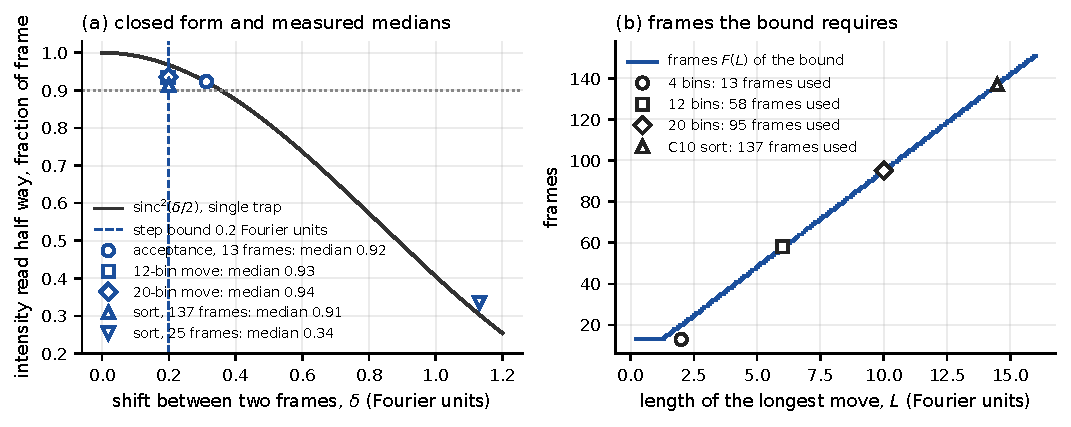
\includegraphics[width=\textwidth]{fig-theory.pdf}
\caption{Theory of the transient intensity. (a) Closed form $\operatorname{sinc}^2(\delta/2)$ of the intensity of a single trap read half way between two frames shifted by $\delta$ Fourier units, with the step bound of the sequence and the median transient minimum ratio measured at the peak steps of the acceptance task (13 frames), the two lattice moves and the sort. (b) Frames that the bound requires against the length of the move, with the frame counts used in the experiments marked.}
\label{fig:theory}
\end{figure}

Figure~\ref{fig:theory} shows both statements. Panel (a) shows that the closed form falls slowly at first, so a small shift costs little and the bound on the step is what keeps the single-trap intensity above $0.9$; the measured points lie below the curve on the long moves, which is the effect of the other traps and of the seeds that fail. It does not show the effect of the weights or the locks, which are measured and not derived. Panel (b) shows that the frame count rises linearly with the move, so the longest rearrangement move needs several times the frames of the acceptance move, which is the practical limit of the method discussed in Section~\ref{sec:discussion}.

\subsection{What the lock guarantees about the phase}

\begin{proposition}\label{prop:lock}
Let $\theta_m(s)$ be the prescribed phase of trap $m$, $\psi_m(s)$ its achieved phase $\arg V_m$ at frame $s$, and $\varepsilon_m(s)=\operatorname{wrap}(\psi_m(s)-\theta_m(s))$ the residual of the iteration. Then
\begin{equation}
\big|\operatorname{wrap}\big(\psi_m(s+1)-\psi_m(s)\big)\big|\le\big|\theta_m(s+1)-\theta_m(s)\big|+|\varepsilon_m(s)|+|\varepsilon_m(s+1)|,\label{eq:lockbound}
\end{equation}
and the largest phase step of Eq.~\ref{eq:phasestep} is at most $\dot\theta_{\max}+2\max_{m,s}|\varepsilon_m(s)|$. With held phases, $\theta_m(s)$ is constant, $\Theta\le2\max|\varepsilon|$, and so $\max|\varepsilon|\ge\Theta/2$.
\end{proposition}
\begin{proof}
Write $\psi_m(s)=\theta_m(s)+\varepsilon_m(s)$ modulo $2\pi$. The wrapped difference of two sums is the wrapped sum of the wrapped differences, and the triangle inequality on the circle gives Eq.~\ref{eq:lockbound}. The second statement follows by taking the maximum and using Eq.~\ref{eq:phasebound}. With held phases the first term of the right-hand side is zero, so $\Theta\le2\max|\varepsilon|$.
\end{proof}

Two consequences follow. First, under the lock the phase step is controlled by two quantities, a prescribed one that the user sets and a residual that the iteration leaves, and the residual shrinks as the weighted iteration converges; without the lock there is no prescribed quantity and no control on the step, only the empirical smallness of the change that the induction of Kim et al.\ assumes. Second, the measured step of the sequence on the acceptance task, \accBStepMax{} rad with held phases, is therefore at most twice the largest residual, and by the last statement of the proposition the largest residual phase error over the moving traps and frames of at least one seed is at least \fpeval{round(\accBStepMax/2,3)} rad. The lock does not remove the phase step; it reduces it to the residual of the iteration. This is the statement that Section~\ref{sec:ablation} tests by removing the lock.

\begin{conjecture}\label{conj:phasepath}
When the sequence misses the intensity floor on a long move with the frames of Eq.~\ref{eq:frames}, the cause is the phase path that the end phases prescribe, not the number of frames or the number of iterations per frame.
\end{conjecture}
The evidence is that the seeds that miss the floor on the lattice moves stay below it when the frames are doubled: with the frames of the bound the failing seeds reach \longFailList{}, and with twice the frames \longTwiceList{}. The conjecture would be refuted by a seed that misses the floor with the frames of the move and reaches it with more frames or iterations; the data of this paper contain none. The conditions under which the end phases from the phase-fixed weighted algorithm give a good path are not characterized.

\section{Experimental design}\label{sec:design}

\subsection{Hypotheses}

The hypotheses are stated here, before the results, with the condition that refutes each; Table~\ref{tab:hyp} lists them. H1, H5, H6 and H7 are the thresholds that the sequence was designed against: a transient ratio of $0.9$ on the acceptance task, on longer moves with the frames of Eq.~\ref{eq:frames}, and the rationale of its two components, the lock and the per-frame optimization. They were fixed with the method and before the comparison with the per-frame sequence existed. H2 to H4 compare the sequence with the per-frame Gerchberg--Saxton sequence of Kim et al.~\cite{kimoe} and were stated after the sequence was designed, when that method was added to the comparison; they are post hoc with respect to the design of the method, and their thresholds come from the benchmark rule of Section~\ref{sec:stats}. The comparison with the linear time profile was added after the results and is not one of the hypotheses: it is reported as a finding made after the results (Table~\ref{tab:profile}). H8 is the consequence of the frame-count equation for a move given fewer frames than the bound asks.

\begin{table}[t]
\centering\small
\caption{Hypotheses with the condition that refutes each. The comparison hypotheses H2 to H4 are against per-frame Gerchberg--Saxton with phase induction at 5 iterations per frame; the outcome of each is in Table~\ref{tab:outcome}.}
\label{tab:hyp}
\begin{tabular}{@{}l p{6.7cm} p{6.0cm}@{}}
\toprule
ID & Statement & Refuted if\\
\midrule
H1 & On the acceptance task the sequence keeps the lowest moving trap at $0.9$ of its mean or more and above linear phase interpolation & a seed below $0.9$, or the paired interval of the difference includes zero\\
H2 & The largest phase step between frames of the sequence is smaller than that of per-frame Gerchberg--Saxton with phase induction & any seed in which the sequence has the larger step\\
H3 & The transient minimum ratio of the sequence is not lower than that of per-frame Gerchberg--Saxton with phase induction & the benchmark rule reads the dip of the published method as better\\
H4 & The largest per-frame spread of the sequence is not larger than that of the per-frame method & the benchmark rule reads the spread of the published method as better\\
H5 & With the frames of the bound, the sequence keeps the lowest moving trap at $0.9$ or more on a majority of seeds of the long moves and of the sort & a majority of seeds below $0.9$ on a move\\
H6 & Removing the trajectory lock brings the lowest moving trap below $0.9$ & the variant stays at $0.9$ or more on a majority of seeds\\
H7 & Removing the per-frame optimization brings the lowest moving trap below $0.9$ & the variant stays at $0.9$ or more on a majority of seeds\\
H8 & With fewer frames than the default, the transient ratio of the sequence falls below $0.9$ & the median at 7 frames is $0.9$ or more\\
\bottomrule
\end{tabular}
\end{table}

\subsection{Data and tasks}

All data are generated by the engine from seeds; no measured hologram or camera image enters the paper. The setup is the one of Section~\ref{sec:problem}. The acceptance task is a $4\times4$ lattice of equal traps eight bins apart in which the two right-hand columns, eight traps, move four bins in $x$; it is run at \parFrames{} frames, the default, and at $7$ and $25$ frames, with \nSeedsTwo{} seeds each. The long lattice moves are the same lattice with the two columns moved \longABins{} and \longBBins{} bins on a 64-pixel SLM, run at the frames of the bound (\longAFrames{} and \longBFrames{}) with \longSeeds{} seeds, and, where a seed fails, at twice that count. The sort is the rearrangement case of the studio: a $6\times6$ array in which \cTenMoving{} of \cTenTraps{} targets are reached by a move, with the assignment of the Hungarian method of Lee et al.~\cite{lee2017}; its longest move is \cTenFu{} Fourier units and it is run at \cTenEqual{} frames and at the \cTenFrames{} frames of the bound with \cTenSeeds{} seeds. The assignment returned by the rearrangement method differs from the plan of the case on ties, so every sequence of the sort runs on the assignment that the rearrangement method returns, and all methods move the same traps along the same paths. The ablation uses the acceptance task at \parFrames{} frames and \ablTN{} seeds.

\subsection{Methods compared}

Three sequences are run on every task. The sequence under test is the flicker-bounded sequence of Section~\ref{sec:flicker-method} with \parFrameIters{} iterations per frame. The first baseline is linear phase interpolation as described by Knottnerus et al.~\cite{lpi}: two phase-fixed weighted Gerchberg--Saxton holograms of \setupCold{} iterations for the endpoints, the position, amplitude and optical phase of each trap read from their fields and interpolated linearly over the frames (the phase by its wrapped difference), and the transform inverted at every frame without optimization. It is our implementation of a published description, not the authors' code. The second baseline is the per-frame sequence of Kim et al.~\cite{kimoe}, implemented in the engine as an option of the rearrangement method and shown as Algorithm~\ref{alg:kim}: frame 0 is the cold run of \setupCold{} iterations, and every later frame starts from the phase of the previous frame and runs a fixed number of weighted iterations toward the trap positions of that frame. It is run at \parKimIters{} iterations per frame, the count of the numerical experiment of Kim et al., and at \parFrameIters{}, the count of the proposed sequence, so that the two are also compared at equal work per frame. The weights of the feedback restart at 1 in every frame in this implementation; only the phase is carried. The paper's phase-change reduction is not implemented, because the authors did not use it in their experiments either. Both baselines use the linear constant-velocity trajectory of the rearrangement method. The proposed sequence is run with two time profiles, stated as a parameter of every comparison: its default, the minimal-jerk profile, and the linear profile of the baselines; Table~\ref{tab:profile} reads both against every baseline by the rule below. Two deviations from the paper of Kim et al.\ remain in the baseline. The zero-padding factor of the setup is \setupPad{}, while their Fig.~3 uses 4. Their frame 0 is a weighted Gerchberg--Saxton run from a random-superposition start, with a random stream of its own, whereas frame 0 of the proposed sequence is the phase-fixed rule~\cite{kimol}.

\begin{algorithm}[t]
\caption{Per-frame Gerchberg--Saxton with phase induction (Kim et al.), as run by the engine, for frames at the trap sets $X(0),\dots,X(S)$ on a linear trajectory.}
\label{alg:kim}
\begin{algorithmic}[1]
\Require traps $X(s)$ for $s=0,\dots,S$, iterations $K_0$ for frame 0, iterations $K$ per later frame, seed
\Ensure holograms $\phi^{(0)},\dots,\phi^{(S)}$
\State $\phi^{(0)}\gets$ weighted GS of $K_0$ iterations on $X(0)$ from a random-superposition start
\For{$s=1,\dots,S$}
  \State $\phi\gets\phi^{(s-1)}$ \Comment{induction: the previous phase is the initial phase}
  \State $w_m\gets1$
  \For{$t=1,\dots,K$}
    \State $V_m\gets V_m(\phi)$ at $x_m(s)$; $w_m\gets w_m\langle r\rangle/r_m$; $\phi\gets\arg\sum_mw_ma_m\,e^{i\arg V_m}\,e^{+i\Delta^m}$
  \EndFor
  \State $\phi^{(s)}\gets\phi\bmod2\pi$
\EndFor
\State \Return $\phi^{(0)},\dots,\phi^{(S)}$
\end{algorithmic}
\end{algorithm}

The difference between Algorithm~\ref{alg:kim} and Algorithm~\ref{alg:flicker} is in two lines: the phase of each coefficient is the current field's phase, free to move, and the weights restart, against the prescribed phase and the carried weights of the proposed sequence. All three sequences are scored by one function that computes Eqs.~\ref{eq:transient} to~\ref{eq:sigmaframe} from the frames and the trajectory, so that no sequence is scored on its own model.

\subsection{Metrics and statistics}\label{sec:stats}

The metrics are the transient minimum ratio $\rho$ of Eq.~\ref{eq:transient}, the per-frame minimum ratio, the largest phase step $\Theta$ of Eq.~\ref{eq:phasestep}, the largest per-frame spread $\sigma_{\max}$ of Eq.~\ref{eq:sigmaframe}, the number of frames against the frame-count equation, and the seconds of a run. The transient ratio of a method is summarized by the mean, the sample standard deviation and the interval of the mean over $n$ seeds,
\begin{equation}
\bar\rho\pm t_{n-1}\frac{s}{\sqrt n},\qquad s^2=\frac1{n-1}\sum_i\big(\rho_i-\bar\rho\big)^2,\label{eq:ci}
\end{equation}
with $t_{n-1}$ the two-sided 95 percent quantile of Student's $t$ distribution, and the comparison of the sequence with a baseline on the same seed index is the paired difference
\begin{equation}
\Delta_i=\rho_i^{\mathrm{seq}}-\rho_i^{\mathrm{base}},\qquad \bar\Delta\pm t_{n-1}\frac{s_\Delta}{\sqrt n}.\label{eq:paired}
\end{equation}
The pairing is by seed index only: the proposed sequence draws its random start from the seed, and the baselines draw theirs from an offset seed, so the methods do not share a random start and the paired interval is not a matched-start comparison. With $n$ of six or eight the intervals are wide and the tests that they imply have low power; no $p$-value is reported, and a claim rests on the interval, the count of seeds that meet a threshold and the reading rule below. Medians and ranges are reported as well because the distributions are not normal.

The reading of a comparison, which method is better on a measure, is the rule of the studio's benchmark and is applied identically to every cell: at least \winMinSeeds{} seeds on both sides, interquartile ranges that do not overlap, and a gap of at least \winMinDiff{} percentage points of the dip below the mean, $100(1-\rho)$, which is lower for the better method, or of the per-frame spread; otherwise the cells are read as a tie. The word \emph{proposed} in a table reads the sequence as better by this rule, \emph{published} reads the baseline as better, and \emph{tie} reads neither. The rule is conservative: a difference in the mean can be real and read as a tie.

\subsection{Protocol}

Every method is deterministic given a seed through the portable generator of the engine, so a rerun reproduces the numbers up to the floating point of the machine's FFT; the seconds differ between runs. The seeds are $1,\dots,n$ with $n$ stated per experiment in the previous subsections. The seconds are wall-clock times of one run of the sequence on the machine that produced the data, with another job loading the machine during part of the runs, so they are reported as an order of magnitude and not as a benchmark. The ablation removes one component at a time and keeps the others, on the same seeds and task as the main result, and the variant with all components is checked against the module of the engine (Section~\ref{sec:flicker-method}). The tables of the results are written by the same script that runs the experiments, from the stored measurement file, so that a table cannot differ from the figure drawn from the same file. Every comparison reports the number of seeds on each side, since the reading rule needs at least \winMinSeeds{} on both.

\section{Results}\label{sec:results}

\subsection{The acceptance task at the default number of frames}

Table~\ref{tab:main} gives the main comparison on the acceptance task with \parFrames{} frames over \nSeedsTwo{} seeds, and Fig.~\ref{fig:curves} shows the intensity of the lowest moving trap along one sequence.

\begin{table}[t]
\centering\small
\caption{Acceptance task, \parFrames{} frames, \nSeedsTwo{} seeds: transient minimum ratio of the moving traps (mean and 95 percent interval of the mean), per-frame minimum ratio (median), largest phase step (maximum over the seeds), largest per-frame spread (median over the seeds), seconds per sequence (median) and the reading of the benchmark rule against the flicker-bounded sequence on the dip.}
\label{tab:main}
\adjustbox{max width=\textwidth}{\begin{tabular}{@{}l r r r r r r@{}}
\toprule
Sequence & Transient minimum ratio, mean (95\% interval) & Per-frame minimum ratio & Largest phase step (rad) & Largest frame $\sigma$ (\%) & Seconds & Reading against the flicker-bounded sequence \\
\midrule
flicker-bounded sequence & 0.923 (0.916 to 0.930) & 0.987 & 0.077 & 0.24 & 1.19 &  \\
linear phase interpolation & 0.644 (0.584 to 0.703) & 0.652 & 0.476 & 23.50 & 1.63 & proposed ($n$ = 6, 6) \\
per-frame GS with phase induction, 5 iterations & 0.948 (0.929 to 0.966) & 0.973 & 0.408 & 2.23 & 0.59 & published ($n$ = 6, 6) \\
per-frame GS with phase induction, 10 iterations & 0.925 (0.890 to 0.961) & 0.981 & 0.619 & 1.29 & 0.94 & tie ($n$ = 6, 6) \\
\bottomrule
\end{tabular}
}
\end{table}

\begin{figure}[t]
\centering
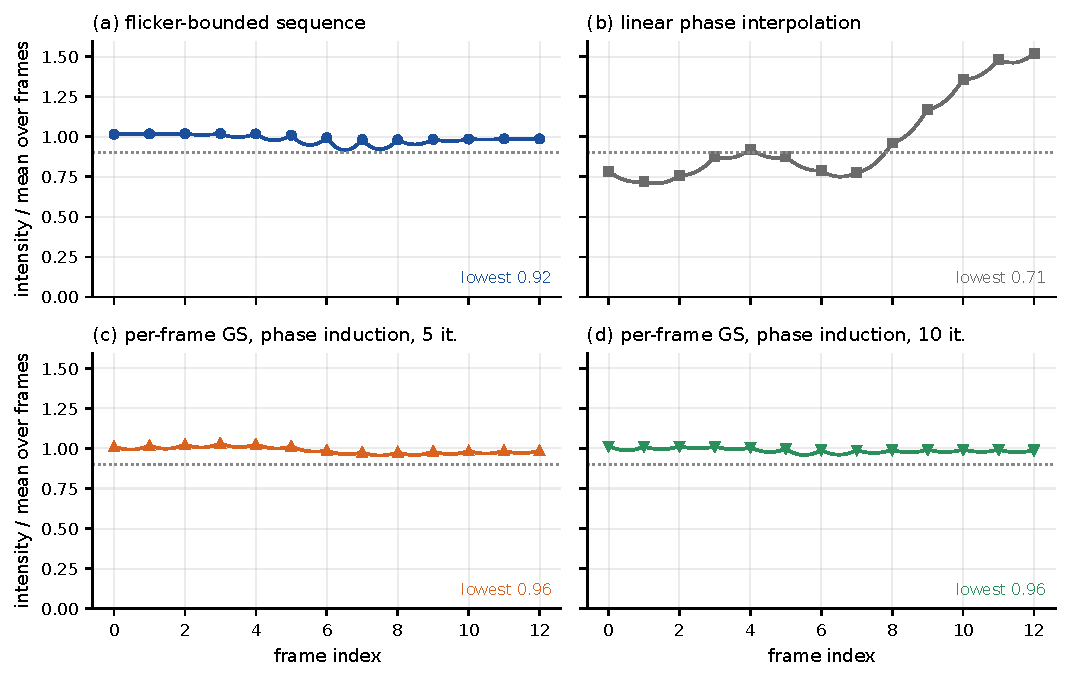
\includegraphics[width=\textwidth]{fig-curves.pdf}
\caption{Intensity of the lowest moving trap of each method, divided by its mean over the frames, along the \parFrames{}-frame acceptance sequence of the first seed: frames are the markers and the lines between them are the blend of two holograms. The dotted line is $0.9$. Linear phase interpolation (b) dips and overshoots; the three optimized sequences (a, c, d) stay close to one, and the per-frame sequences show small steps at the frames.}
\label{fig:curves}
\end{figure}

For the sequence the lowest transient ratio of the moving traps is a mean of \accBTransMean{} (standard deviation \bTwoSd{}, interval \accBTransCiLo{} to \accBTransCiHi{}, median \accBTransMed{}, range \accBTransMin{} to \accBTransMax{}), above $0.9$ on every seed. Linear phase interpolation has a mean of \accLpiTransMean{} (standard deviation \lpiSd{}, interval \accLpiTransCiLo{} to \accLpiTransCiHi{}, range \accLpiTransMin{} to \accLpiTransMax{}), below $0.9$ on every seed. The paired difference of Eq.~\ref{eq:paired} has a mean of \diffTwoMean{} with a 95 percent interval of \diffTwoCiLo{} to \diffTwoCiHi{}, so the interval excludes zero, and the benchmark rule reads the dip as \readThirteenLpiDip{} for the sequence ($n$ = \readThirteenLpiDipN). The per-frame spread differs by a factor of \sigmaFrameFactorLo{} to \sigmaFrameFactorHi{}: the largest per-frame relative standard deviation is at most \bTwoSigmaFrame{} percent for the sequence (median \bTwoSigmaFrameMed{}) and between \lpiSigmaFrameMin{} and \lpiSigmaFrameMax{} percent for linear phase interpolation (median \lpiSigmaFrameMed{}), because its intermediate frames are not optimized.

The per-frame Gerchberg--Saxton sequence with phase induction at \parKimIters{} iterations per frame reaches a higher minimum than the proposed sequence: a mean of \accKimFiveTransMean{} (interval \accKimFiveTransCiLo{} to \accKimFiveTransCiHi{}, range \accKimFiveTransMin{} to \accKimFiveTransMax{}) against \accBTransMean{}, a gap of \dipGap{} in the mean, and the benchmark rule reads the dip as \readThirteenKimFiveDip{} ($n$ = \readThirteenKimFiveDipN). On every seed the published method is above the proposed sequence on this measure. At equal work, \parFrameIters{} iterations per frame, its mean is \accKimTenTransMean{} (interval \accKimTenTransCiLo{} to \accKimTenTransCiHi{}) and the rule reads a \readThirteenKimTenDip{}. So the finding for the dip is: the proposed sequence is well above linear phase interpolation, below the published per-frame method at its own iteration count, and indistinguishable from it at ten iterations per frame. On the per-frame spread the reading is \readThirteenKimFiveSigma{} for the sequence against the per-frame method at \parKimIters{} iterations and \readThirteenKimTenSigma{} at ten: its frames are better equalized, with a median largest spread of \accBSigmaMed{} percent against \accKimFiveSigmaMed{} and \accKimTenSigmaMed{} percent.

\begin{table}[t]
\centering\small
\caption{The time profile of the sequence as a parameter, a comparison added after the results, acceptance task, \parFrames{} frames, \readProfileN{} seeds: transient minimum ratio (mean and 95 percent interval), largest phase step (maximum over seeds), largest per-frame spread (median) and the reading of the benchmark rule against each baseline on the dip, for the default minimal-jerk profile and for the linear profile of the baselines.}
\label{tab:profile}
\adjustbox{max width=\textwidth}{\begin{tabular}{@{}l r r r l l l@{}}
\toprule
Time profile of the sequence & Transient minimum ratio, mean (95\% interval) & Largest phase step (rad) & Largest frame $\sigma$ (\%) & Reading against per-frame GS, 5 iterations & Against 10 iterations & Against linear phase interpolation \\
\midrule
minimal-jerk (the default) & 0.923 (0.916 to 0.930) & 0.077 & 0.24 & published ($n$ = 6, 6) & tie ($n$ = 6, 6) & proposed ($n$ = 6, 6) \\
linear (the baselines' profile) & 0.967 (0.960 to 0.974) & 0.086 & 0.21 & proposed ($n$ = 6, 6) & proposed ($n$ = 6, 6) & proposed ($n$ = 6, 6) \\
\bottomrule
\end{tabular}
}
\end{table}

Table~\ref{tab:profile} reports both time profiles against every baseline. With the default minimal-jerk profile the rule reads the dip as \readProfileDefaultKimFiveDip{} against the per-frame method at \parKimIters{} iterations, as a \readProfileDefaultKimTenDip{} at \parFrameIters{} iterations and as \readProfileDefaultLpiDip{} against linear phase interpolation. With the linear profile it reads \readProfileLinearKimFiveDip{} against the per-frame method at \parKimIters{} iterations, \readProfileLinearKimTenDip{} at \parFrameIters{} and \readProfileLinearLpiDip{} against linear phase interpolation, on the dip and on the per-frame spread alike, with a mean of \ablTLinearMean{} against \accKimFiveTransMean{}. The deficit of the default profile has a cause that the data locate: at \parFrames{} frames its peak shift between frames is \accPeakStep{} Fourier units, outside the method's own step bound of \claimStepFu{} Fourier units, for which the bound asks \accFramesForMove{} frames, while the constant-velocity profile at the same frame count has a smaller peak shift for the same move. The default therefore runs outside the bound that the paper derives, and the comparison at this frame count sets the sequence outside its design condition against baselines inside theirs. At 25 frames, inside the bound, the default ties both per-frame sequences (Table~\ref{tab:frames}).

\subsection{Number of frames}

\begin{table}[t]
\centering\small
\caption{Transient minimum ratio of the moving traps (median and range over \nSeedsTwo{} seeds) and per-frame minimum ratio (median) of the four sequences on the acceptance task at 7, \parFrames{} and 25 frames.}
\label{tab:frames}
\adjustbox{max width=\textwidth}{\begin{tabular}{@{}l l r r r r@{}}
\toprule
Frames & Sequence & Transient minimum ratio, median & Range & Per-frame minimum ratio, median & $n$ \\
\midrule
13 & flicker-bounded sequence & 0.923 & 0.915 to 0.932 & 0.987 & 6 \\
13 & linear phase interpolation & 0.648 & 0.551 to 0.709 & 0.652 & 6 \\
13 & per-frame GS with phase induction, 5 iterations & 0.953 & 0.918 to 0.965 & 0.973 & 6 \\
13 & per-frame GS with phase induction, 10 iterations & 0.926 & 0.880 to 0.966 & 0.981 & 6 \\
7 & flicker-bounded sequence & 0.754 & 0.735 to 0.766 & 0.986 & 6 \\
7 & linear phase interpolation & 0.621 & 0.479 to 0.666 & 0.663 & 6 \\
7 & per-frame GS with phase induction, 5 iterations & 0.896 & 0.877 to 0.903 & 0.976 & 6 \\
7 & per-frame GS with phase induction, 10 iterations & 0.868 & 0.794 to 0.895 & 0.975 & 6 \\
25 & flicker-bounded sequence & 0.973 & 0.963 to 0.977 & 0.988 & 6 \\
25 & linear phase interpolation & 0.648 & 0.576 to 0.722 & 0.651 & 6 \\
25 & per-frame GS with phase induction, 5 iterations & 0.970 & 0.934 to 0.980 & 0.972 & 6 \\
25 & per-frame GS with phase induction, 10 iterations & 0.949 & 0.891 to 0.982 & 0.981 & 6 \\
\bottomrule
\end{tabular}
}
\end{table}

\begin{figure}[t]
\centering
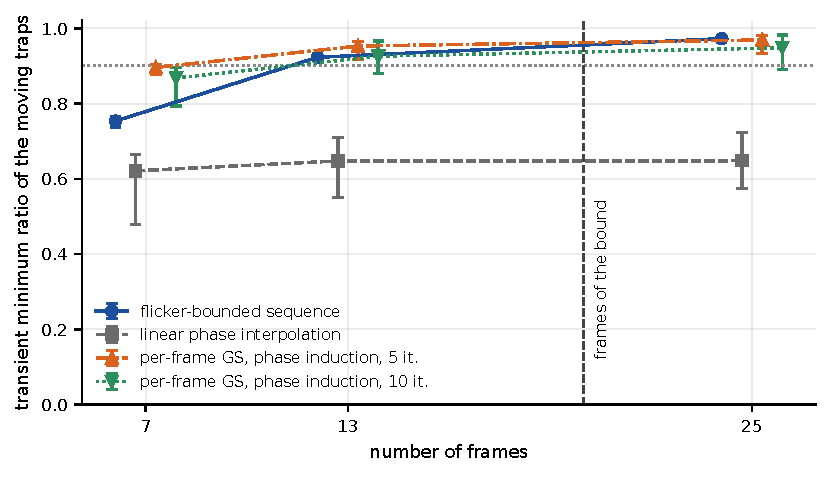
\includegraphics[width=\textwidth]{fig-frames.pdf}
\caption{Transient minimum ratio of the moving traps against the number of frames of the acceptance task for the four sequences; markers are medians over \nSeedsTwo{} seeds and bars are the range. The dotted line is $0.9$ and the dashed vertical line is the number of frames that the bound of Eq.~\ref{eq:frames} requires for this move.}
\label{fig:frames}
\end{figure}

Table~\ref{tab:frames} and Fig.~\ref{fig:frames} vary the number of frames. With 7 frames the sequence reaches a median of \bTwoMedSeven{} (minimum \bTwoMinSeven), below $0.9$ on every seed, linear phase interpolation \lpiMedSeven{}, and the per-frame method at \parKimIters{} iterations \readSevenKimFiveDip{} by the rule and at ten iterations \readSevenKimTenDip{}: with few frames the induced sequence is clearly better than the proposed one, which is consistent with the frame-count equation, because the move of two Fourier units needs \accFramesForMove{} frames for the step bound and 7 frames give a peak step of \fpeval{round(15/8*\accFu/(7-1)/\claimStepFu,1)} times the bound. With 25 frames, above the bound for this move, the sequence reaches a median of \bTwoMedTwentyFive{} (minimum \bTwoMinTwentyFive), linear phase interpolation \lpiMedTwentyFive{}, and the reading against both per-frame sequences is a \readTwentyFiveKimFiveDip{} and a \readTwentyFiveKimTenDip{}. The proposed sequence thus gains more from extra frames than linear phase interpolation, which does not improve, and catches up with the per-frame method; the per-frame method is the better choice when the number of frames is small and the two are equivalent on this measure when it is large. The per-frame minimum ratio, without the blend, is above $0.97$ for the sequence and the per-frame sequences at all three counts, so the dips of the first three are produced by the transition between frames and not by the frames.

\subsection{Phase continuity}

\begin{figure}[t]
\centering
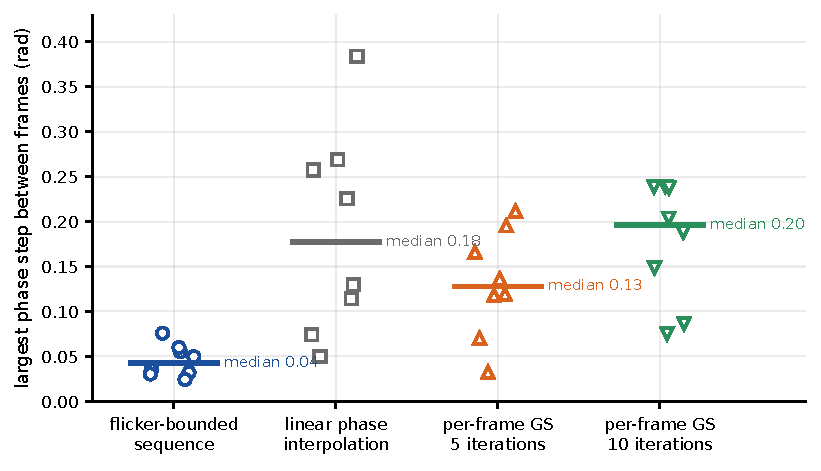
\includegraphics[width=\textwidth]{fig-steps.pdf}
\caption{Largest phase step between consecutive frames of each of the eight moving traps of the acceptance task (first seed), for the four sequences. Each marker is one trap and the horizontal lines are the medians over the traps, lowest for the sequence. The ranges of the traps overlap between methods, so the comparison of the text rests on the largest step of each seed (Table~\ref{tab:main}), which is at the top of each column.}
\label{fig:steps}
\end{figure}

Figure~\ref{fig:steps} shows the quantity that the lock is designed to control, the largest phase step $\Theta$ of Eq.~\ref{eq:phasestep}. Over the \nSeedsTwo{} seeds of the acceptance task the largest phase step of the sequence is \accBStepMax{} rad (mean \accBStepMean{}, interval \accBStepCiLo{} to \accBStepCiHi{}). The per-frame method at \parKimIters{} iterations has \accKimFiveStepMax{} rad (mean \accKimFiveStepMean{}), a factor of \stepRatio{}; at ten iterations it has \accKimTenStepMax{} rad, a factor of \stepRatioTen{}; and linear phase interpolation has \accLpiStepMax{} rad, a factor of \stepRatioLpi{}. The sequence has the smaller step on every one of the \nSeedsTwo{} seeds against the per-frame method at \parKimIters{} iterations, and the same holds at 7 and 25 frames. Two readings of these numbers are limited. The step of linear phase interpolation is not small even though its interpolated phase is linear, because the phase achieved in a frame that is an inverse transform of interpolated spots is not the interpolated one. And the largest step of the induced sequence, \accKimFiveStepMax{} rad, is about \fpeval{round(\accKimFiveStepMax/pi,2)}$\pi$, below the several tenths of $\pi$ at which Knottnerus et al.\ saw no change in atom survival~\cite{lpi}: the measurements do not show that the induced sequence would lose atoms. The advantage of the lock is a margin on a quantity that matters near $\pi$, and the acceptance task does not approach it.

\subsection{Long moves and the sort of a \texorpdfstring{$6\times6$}{6 by 6} array}

\begin{table}[t]
\centering\small
\caption{Transient minimum ratio of the moving traps on the long lattice moves ($\longSeeds$ seeds) and on the sort of the $6\times6$ array ($\cTenSeeds$ seeds), each at the frames of the bound: median and range over seeds, seeds at $0.9$ or above, and the reading of the benchmark rule against the flicker-bounded sequence.}
\label{tab:long}
\adjustbox{max width=\textwidth}{\begin{tabular}{@{}l r l r r r r@{}}
\toprule
Move & Frames & Sequence & Median & Range & Seeds at 0.9 or above & Reading against the flicker-bounded sequence \\
\midrule
lattice, 12 bins & 58 & flicker-bounded sequence & 0.933 & 0.023 to 0.965 & 6 of 8 &  \\
lattice, 12 bins & 58 & linear phase interpolation & 0.675 & 0.568 to 0.756 & 0 of 8 & proposed ($n$ = 8) \\
lattice, 12 bins & 58 & per-frame GS with phase induction, 5 iterations & 0.960 & 0.927 to 0.976 & 8 of 8 & tie ($n$ = 8) \\
lattice, 12 bins & 58 & per-frame GS with phase induction, 10 iterations & 0.948 & 0.912 to 0.978 & 8 of 8 & tie ($n$ = 8) \\
lattice, 20 bins & 95 & flicker-bounded sequence & 0.936 & 0.584 to 0.966 & 6 of 8 &  \\
lattice, 20 bins & 95 & linear phase interpolation & 0.651 & 0.581 to 0.701 & 0 of 8 & proposed ($n$ = 8) \\
lattice, 20 bins & 95 & per-frame GS with phase induction, 5 iterations & 0.960 & 0.928 to 0.976 & 8 of 8 & published ($n$ = 8) \\
lattice, 20 bins & 95 & per-frame GS with phase induction, 10 iterations & 0.949 & 0.908 to 0.979 & 8 of 8 & tie ($n$ = 8) \\
rearrangement C10, 16 moving traps & 137 & flicker-bounded sequence & 0.914 & 0.909 to 0.917 & 6 of 6 &  \\
rearrangement C10, 16 moving traps & 137 & linear phase interpolation & 0.556 & 0.044 to 0.738 & 0 of 6 & proposed ($n$ = 6) \\
rearrangement C10, 16 moving traps & 137 & per-frame GS with phase induction, 5 iterations & 0.938 & 0.922 to 0.956 & 6 of 6 & published ($n$ = 6) \\
rearrangement C10, 16 moving traps & 137 & per-frame GS with phase induction, 10 iterations & 0.920 & 0.846 to 0.936 & 5 of 6 & tie ($n$ = 6) \\
\bottomrule
\end{tabular}
}
\end{table}

\begin{figure}[t]
\centering
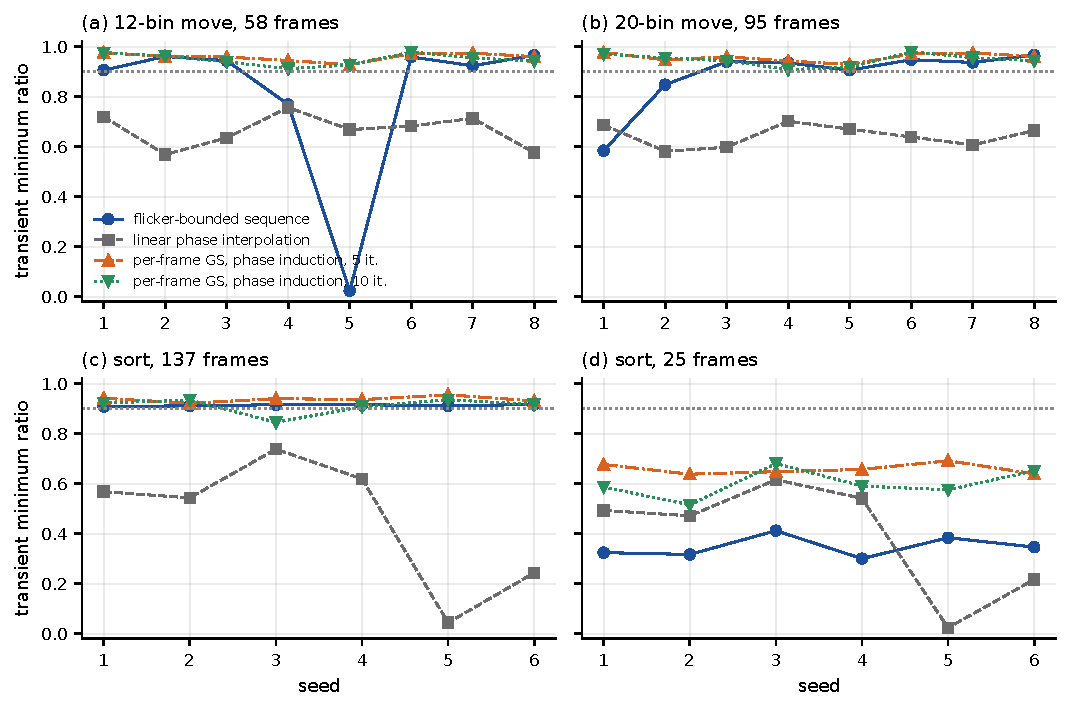
\includegraphics[width=\textwidth]{fig-long.pdf}
\caption{Transient minimum ratio of the moving traps per seed for the four sequences on (a) the 12-bin lattice move at 58 frames, (b) the 20-bin move at 95 frames, (c) the sort at the 137 frames of the bound and (d) the sort at 25 frames. Each line connects the seeds of one method; the dotted line is $0.9$.}
\label{fig:long}
\end{figure}

Table~\ref{tab:long} and Fig.~\ref{fig:long} give the moves that the bound was made for. With the frames of the bound the sequence reaches a median of \longAMed{} on the 12-bin move and \longBMed{} on the 20-bin move, with \longAMet{} of \longSeeds{} seeds at $0.9$ or above on each, and \cTenMet{} of \cTenSeeds{} on the sort, with a median of \cTenMetMed{} and a range of \cTenMetMin{} to \cTenMetMax{}. Linear phase interpolation reaches $0.9$ on none (range \longALpiMin{} to \longALpiMax{} and \longBLpiMin{} to \longBLpiMax{} on the lattice moves, \cTenLpiMin{} to \cTenLpiMax{} on the sort), and the sequence is above it on \longABLeadsLpi{} of \longSeeds{} seeds of each lattice move and on \cTenBLeads{} of \cTenSeeds{} of the sort. The two seeds of each lattice move that fail do so by a wide margin: \longFailList{}. Doubling the frames does not rescue them (\longTwiceList{}), which supports Conjecture~\ref{conj:phasepath}.

The per-frame sequence of Kim et al.\ reaches $0.9$ on every seed of both lattice moves (range \longAKimFiveMin{} to \longAKimFiveMax{} and \longBKimFiveMin{} to \longBKimFiveMax{} at \parKimIters{} iterations) and on every seed of the sort at \parKimIters{} iterations (range \cTenKimFiveMin{} to \cTenKimFiveMax{}). The sequence is above it on \longABLeadsKimFive{} of \longSeeds{} seeds of the 12-bin move, \longBBLeadsKimFive{} of \longSeeds{} of the 20-bin move and \cTenBLeadsKimFive{} of \cTenSeeds{} of the sort. The benchmark rule reads the 12-bin move as a \longAReadKimFive{}, the 20-bin move as \longBReadKimFive{} and the sort as \cTenReadKimFive{} ($n$ = \cTenReadKimFiveN). At ten iterations per frame the readings are \longAReadKimTen{}, \longBReadKimTen{} and \cTenReadKimTen{}. On the sort at the 25 frames of panel (d), where the bound is not met, no method reaches $0.9$; the sequence is at most \cTenBEqualMax{}, linear phase interpolation lies between \cTenLEqualMin{} and \cTenLEqualMax{}, and on every seed both per-frame sequences are above both of them. Without enough frames the per-frame sequences degrade more slowly than the locked one, whose prescribed path forces a large shift between frames.

\begin{table}[t]
\centering\small
\caption{The frame-count equation against the frames used: longest move, frames of the bound, frames used, peak shift per frame, median ratio reached by the flicker-bounded sequence and seeds at $0.9$ or above.}
\label{tab:bound}
\adjustbox{max width=\textwidth}{\begin{tabular}{@{}l r r r r r r@{}}
\toprule
Move & Longest move (Fourier units) & Frames of the bound & Frames used & Peak step (Fourier units) & Ratio reached, median & Seeds at 0.9 or above \\
\midrule
lattice, 4 bins & 2.00 & 20 & 13 & 0.312 & 0.923 & 6 of 6 \\
lattice, 12 bins & 6.00 & 58 & 58 & 0.197 & 0.933 & 6 of 8 \\
lattice, 20 bins & 10.00 & 95 & 95 & 0.199 & 0.936 & 6 of 8 \\
sort of 36 traps (16 moving), 25 frames & 14.48 & 137 & 25 & 1.131 & 0.335 & 0 of 6 \\
sort of 36 traps (16 moving), 137 frames & 14.48 & 137 & 137 & 0.200 & 0.914 & 6 of 6 \\
\bottomrule
\end{tabular}
}
\end{table}

\begin{figure}[t]
\centering
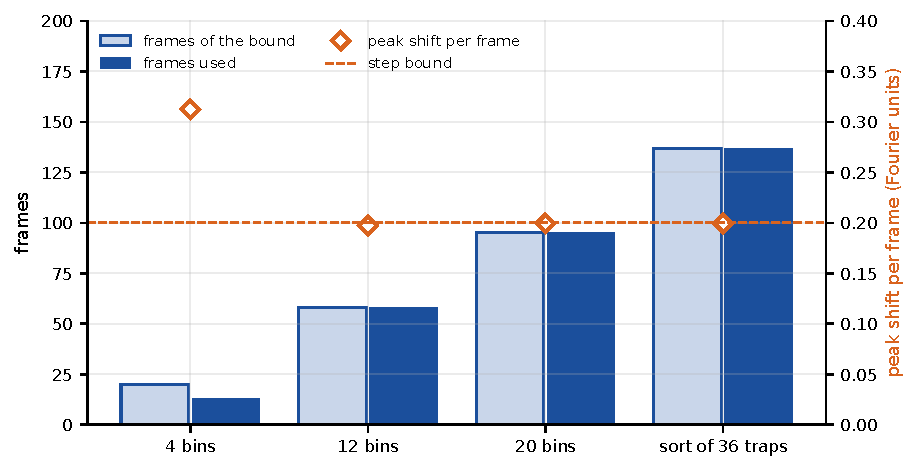
\includegraphics[width=\textwidth]{fig-bound.pdf}
\caption{Frames of the bound and frames used for the four moves of the experiments (acceptance task, two lattice moves and the sort), with the peak shift per frame of the frames used on the right axis; the dashed line is the step bound of the sequence.}
\label{fig:bound}
\end{figure}

Table~\ref{tab:bound} and Fig.~\ref{fig:bound} place the experiments against the equation. The three long moves are run at the frames of the bound and the peak shift per frame is at the bound, \claimStepFu{} Fourier units, up to rounding. The acceptance task is run at \parFrames{} frames, fewer than the \accFramesForMove{} of the bound, with a peak shift of \accPeakStep{} Fourier units, and meets $0.9$ on every seed; the sort at 25 frames has a peak shift of \cTenPeakEqual{} Fourier units and reaches no seed. The bound is therefore sufficient for the median and not necessary for a short move, and it is not sufficient for every seed of a long one.

\subsection{Cost in time}

\begin{figure}[t]
\centering
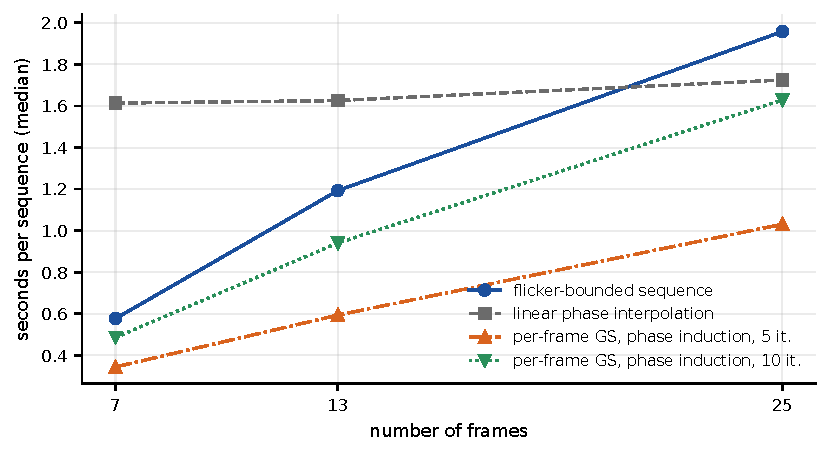
\includegraphics[width=\textwidth]{fig-seconds.pdf}
\caption{Seconds to compute one acceptance sequence of the four methods against the number of frames, median over \nSeedsTwo{} seeds, on the machine that produced the data; other jobs loaded the machine during part of the runs, so the values are an order of magnitude.}
\label{fig:seconds}
\end{figure}

Figure~\ref{fig:seconds} gives the seconds of one sequence. At \parFrames{} frames the median is \accBSecMed{} s for the sequence, \accKimFiveSecMed{} s for the per-frame method at \parKimIters{} iterations, \accKimTenSecMed{} s at ten and \accLpiSecMed{} s for linear phase interpolation, which runs two cold endpoint holograms and no iterations in between. The sequence is \secRatio{} times slower than the per-frame method at its own iteration count, which is the ratio of the iterations per frame, and \fpeval{round(\accBSecMean/\accKimTenSecMean,1)} times slower at equal work. The ratio of the seconds is slightly above the ratio of the iterations of the two sequences, \fpeval{round((\setupCold+(\parFrames-1)*\parFrameIters)/(\setupCold+(\parFrames-1)*\parKimIters),1)}, because the call that computes the proposed sequence also scores its transient ratio on the blend model, which the call of the baselines does not do; the seconds are therefore an upper estimate of the cost of the sequence itself, and they are not a measure of what a deployed implementation would take.

\subsection{Outcome of each hypothesis}

\begin{table}[t]
\centering\small
\caption{Outcome of each hypothesis of Table~\ref{tab:hyp} with the measurement that decides it, and the finding made after the results; ``held'' means the refuting condition did not occur.}
\label{tab:outcome}
\begin{tabular}{@{}l p{3.6cm} p{8.6cm}@{}}
\toprule
ID & Outcome & Measurement\\
\midrule
H1 & held & lowest seed \bTwoMin{}, linear phase interpolation highest seed \lpiMax{}; paired difference \diffTwoMean{} (\diffTwoCiLo{} to \diffTwoCiHi{})\\
H2 & held & largest step \accBStepMax{} rad against minimum \accKimFiveStepMin{} rad over seeds for the per-frame method; the sequence is smaller on every seed\\
H3 & refuted & reading of the dip at the default profile: \readThirteenKimFiveDip{} at \parKimIters{} iterations per frame, \readThirteenKimTenDip{} at \parFrameIters{}\\
H4 & held & reading of the per-frame spread: \readThirteenKimFiveSigma{} at \parKimIters{} iterations, \readThirteenKimTenSigma{} at \parFrameIters{}\\
H5 & held with failures & \longAMet{} of \longSeeds{} and \longBMet{} of \longSeeds{} seeds on the lattice moves, \cTenMet{} of \cTenSeeds{} on the sort\\
H6 & refuted by the majority rule & see Table~\ref{tab:ablation}: a majority of seeds stays at $0.9$ without the lock, with a lower mean and a wider range\\
H7 & held & see Table~\ref{tab:ablation}: no seed reaches $0.9$ without the per-frame optimization\\
H8 & held & median \bTwoMedSeven{} at 7 frames\\
F & finding made after the results, not a hypothesis & with the linear profile of the baselines the dip is read as \readProfileLinearKimFiveDip{} against the per-frame method at \parKimIters{} iterations, \readProfileLinearKimTenDip{} at \parFrameIters{} and \readProfileLinearLpiDip{} against linear phase interpolation (Table~\ref{tab:profile}); acceptance task only\\
\bottomrule
\end{tabular}
\end{table}

Table~\ref{tab:outcome} collects the outcomes of the eight hypotheses and, in its last row, the finding made after the results. Six hypotheses held, one of them with a qualification (H5, on a majority and not on all seeds), and two were refuted: H3, the sequence with its default profile is not as good on the dip as the published per-frame method at its own iteration count, and H6, by the majority rule the lock is not what keeps the dip above $0.9$ on the acceptance task, it acts on the phase step and on the spread of seeds. The finding made after the results is that with the constant-velocity profile of the baselines the sequence is read as better on the dip than every baseline on the acceptance task; it was not predicted, it was not run on the long moves or the sort, and it is reported as a finding and not as a revision of the outcome of H3. The deficit of the default on the dip belongs to its time profile and to a frame count outside its bound, not to the locked phases. The default frame count of the sequence, \parFrames{}, is the count that the source of linear phase interpolation uses for its sort, and it is below the count that the bound asks for the acceptance move.

\section{Ablation}\label{sec:ablation}

\subsection{Variants and what each removes}

The ablation removes one component of the sequence at a time on the acceptance task at \parFrames{} frames over \ablTN{} seeds, with the same seeds as the main result. The variants are: the sequence with all components; the sequence without the trajectory lock, in which the phase of each coefficient is the phase of the current field as in the induced sequence, while the weights are still carried across frames and the positions still follow the minimal-jerk profile; the sequence without the per-frame optimization, in which every frame is the inverse transform of the prescribed spots with unit weights and no iteration, so that only the lock and the profile remain; the sequence with 1 and with 3 iterations per frame instead of \parFrameIters{}; and the sequence with a linear time profile for the positions instead of the minimal-jerk profile, with the same frame count. The two published sequences are reproduced from Table~\ref{tab:main} as references. Table~\ref{tab:ablation} gives the results and Fig.~\ref{fig:ablation} shows them per seed. The variant with all components is checked against the module of the engine and agrees to \ablTCheck{}, so the other rows are the module with parts removed.

\begin{table}[t]
\centering\small
\caption{Ablation of the flicker-bounded sequence on the acceptance task at \parFrames{} frames over \ablTN{} seeds: transient minimum ratio (mean $\pm$ standard deviation, range), seeds at $0.9$ or above, largest per-frame spread and largest phase step (medians over the seeds); the three last rows are the published sequences for reference.}
\label{tab:ablation}
\adjustbox{max width=\textwidth}{\begin{tabular}{@{}l r r r r r@{}}
\toprule
Variant & Minimum ratio, mean $\pm$ s.d. & Range & Seeds at 0.9 or above & Largest frame $\sigma$ (\%) & Largest phase step (rad) \\
\midrule
flicker-bounded sequence, all components & 0.923 $\pm$ 0.007 & 0.915 to 0.932 & 6 of 6 & 0.24 & 0.069 \\
without the trajectory lock & 0.884 $\pm$ 0.055 & 0.776 to 0.924 & 4 of 6 & 2.45 & 0.455 \\
without the per-frame optimization & 0.789 $\pm$ 0.038 & 0.724 to 0.830 & 0 of 6 & 17.67 & 0.064 \\
1 iteration per frame & 0.747 $\pm$ 0.069 & 0.676 to 0.823 & 0 of 6 & 18.62 & 0.063 \\
3 iterations per frame & 0.918 $\pm$ 0.010 & 0.905 to 0.933 & 6 of 6 & 3.50 & 0.066 \\
linear time profile for the positions & 0.967 $\pm$ 0.006 & 0.959 to 0.974 & 6 of 6 & 0.21 & 0.041 \\
linear phase interpolation (reference) & 0.644 $\pm$ 0.057 & 0.551 to 0.709 & 0 of 6 & 23.50 & 0.409 \\
per-frame GS with phase induction, 5 iterations (reference) & 0.948 $\pm$ 0.017 & 0.918 to 0.965 & 6 of 6 & 2.23 & 0.302 \\
per-frame GS with phase induction, 10 iterations (reference) & 0.925 $\pm$ 0.034 & 0.880 to 0.966 & 4 of 6 & 1.29 & 0.499 \\
\bottomrule
\end{tabular}
}
\end{table}

\begin{figure}[t]
\centering
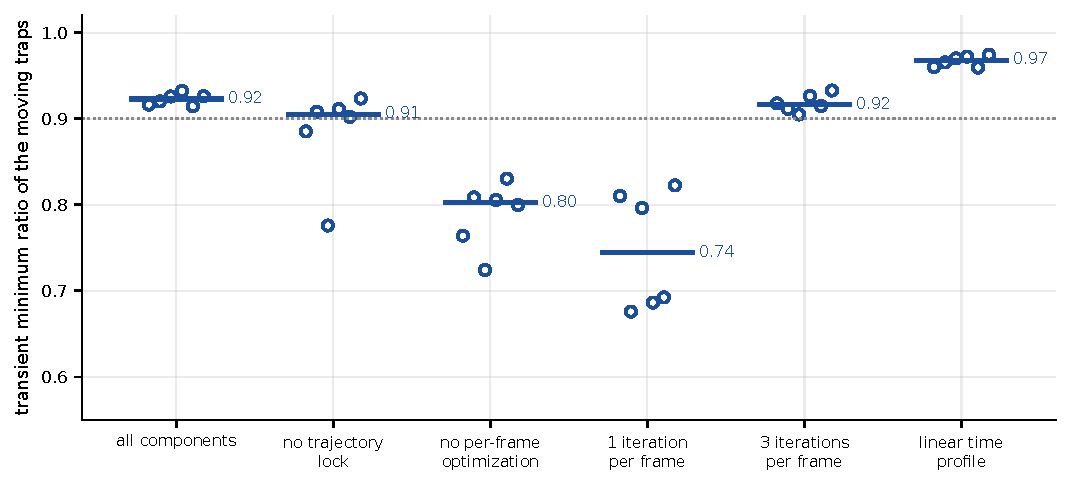
\includegraphics[width=\textwidth]{fig-ablation.pdf}
\caption{Transient minimum ratio of the moving traps per seed for the full sequence and each ablated variant on the acceptance task; markers are seeds, bars are medians, and the dotted line is $0.9$. Removing the per-frame optimization or reducing the iterations to one puts every seed below $0.9$; removing the lock spreads the seeds widely; the linear time profile raises every seed.}
\label{fig:ablation}
\end{figure}

\subsection{Reading the ablation}

\emph{The per-frame optimization is necessary.} Without it the mean falls from \ablTFullMean{} to \ablTNoOptMean{} (standard deviation \ablTNoOptSd{}), no seed reaches $0.9$, and the largest per-frame spread rises from \ablTFullSig{} to \ablTNoOptSig{} percent, close to the \accLpiSigmaMed{} percent of linear phase interpolation. The phase step stays small, \ablTNoOptStep{} rad, since the lock still holds. The variant is better than linear phase interpolation, \accLpiTransMean{}, so the locked phases explain part of the gap to it, and the optimization explains the rest. H7 held.

\emph{The lock does not move the mean as far as the optimization, but it controls the step and the spread of outcomes.} Without the lock the mean is \ablTNoLockMean{} (standard deviation \ablTNoLockSd{}, range \ablTNoLockMin{} to \ablTNoLockMax{}) against \ablTFullMean{} (\ablTFullSd{}), and a majority of seeds still reaches $0.9$, so H6 is refuted by the rule fixed in advance. What changes is the phase step, from \ablTFullStep{} to \ablTNoLockStep{} rad, a factor of \lockStepRatio{}, and the largest spread of a frame, from \ablTFullSig{} to \ablTNoLockSig{} percent. The unlocked variant has the phase step of the induced sequences: \ablTNoLockStep{} rad against the median of \accKimTenStepMed{} rad for the per-frame method at the same iteration count. This is the evidence that the lock, and not the carried weights or the profile, is what reduces the step, and it is the consistency check of Proposition~\ref{prop:lock}.

\emph{Three iterations suffice.} With 3 iterations per frame the mean is \ablTItersThreeMean{}, indistinguishable from \ablTFullMean{} at ten, while with one iteration it falls to \ablTItersOneMean{}. The iteration count of the main experiments, \parFrameIters{}, is therefore conservative for this task, and a sequence with 3 iterations per frame does less work than the per-frame method at \parKimIters{} iterations while reaching a similar level, \ablTItersThreeMean{} against \accKimFiveTransMean{}. Because the experiments of the paper use \parFrameIters{} for the proposed sequence, the comparison with the per-frame method at 5 iterations is in fact favourable to the per-frame method on work, and the comparison at \parFrameIters{} is the equal-work one.

\emph{The minimal-jerk profile lowers the transient minimum on this task.} With a linear time profile and the same number of frames the mean rises to \ablTLinearMean{} (range \ablTLinearMin{} to \ablTLinearMax{}), above the per-frame method at \parKimIters{} iterations by \linearGap{} in the mean, and the median of the largest phase step is \ablTLinearStep{} rad. Table~\ref{tab:profile} reads this variant by the benchmark rule against every baseline: it is better on the dip and on the spread than the per-frame method at both iteration counts and than linear phase interpolation. The reason is Proposition~\ref{prop:frames}: the minimal-jerk profile has a peak velocity of $15/8$ times the mean, so at the same frame count its peak shift between frames is almost twice that of the linear profile, and the transient ratio depends on the peak shift. The minimal-jerk profile is the default for a reason that concerns the motion of atoms and that the cited experiment supports only for a different system (Section~\ref{sec:flicker-method}); the hologram measurements here do not weigh that reason, and they score the linear profile higher on every measure of the table.

Taken together, the ablation says that the value of the sequence lies in the combination of the lock with the per-frame optimization, that the lock is what lowers the phase step, that three iterations per frame suffice on this task, and that the time profile is a parameter that decides the reading against the published per-frame method: the default minimal-jerk profile loses the dip to it at the frame count of the acceptance task, and the linear profile wins. These are the conclusions that Section~\ref{sec:discussion} draws on.

\section{Discussion}\label{sec:discussion}

\subsection{Why the sequences behave as they do}

The transient ratio of Eq.~\ref{eq:transient} falls when two consecutive frames place a moving trap at positions whose fields interfere with a phase difference. Three things control it: the shift of the pattern between frames, which Proposition~\ref{prop:blend} turns into a closed form; the phase of the trap in the two frames, which the lock prescribes and the induction only initializes; and the uniformity of each frame, which the optimization supplies. Linear phase interpolation controls the second and not the third, and it has the lowest ratio of the three sequences because its frames are not equalized: the per-frame spread of its frames is of the order of \lpiSigmaFrameMed{} percent. The per-frame method controls the third and not the second, and in these experiments the induced phases turn out to move by at most \accKimFiveStepMax{} rad between frames, which is small enough for the blend to stay above $0.9$ on every seed at \parFrames{} frames. The proposed sequence controls both, and that is the reason it improves on linear phase interpolation by \diffTwoMean{} in the mean of the ratio. It does not improve on the induced sequence, because the second control is already adequate there.

The direction of the remaining difference needs an explanation. The induced sequence has the higher dip although its phase step is about \stepRatio{} times larger. An explanation consistent with the data is that the transient ratio depends on the shift of the pattern between frames, which differs between the two methods because they follow different time profiles: the baselines move at constant velocity, the proposed sequence moves with a peak velocity of $15/8$ times the mean. The ablation supports this reading: with a linear profile the sequence reaches \ablTLinearMean{}, above the induced sequence at \accKimFiveTransMean{}, and with the profile of the method it is below it. The comparison of the two methods on the dip is therefore partly a comparison of two time profiles and not only of two ways of computing the frames. We report the comparison as run, with the profile that each method was defined with, and the result with the linear profile as an ablation of the proposed sequence.

\subsection{What the lock buys and what it costs}

The lock buys a controlled phase step. Without it the median of the largest step is \ablTNoLockStep{} rad, the value of the induced sequences; with it, \ablTFullStep{} rad, a reduction by a factor of \lockStepRatio{} at equal iterations. It also narrows the spread of outcomes across seeds: the standard deviation of the ratio is \ablTFullSd{} with the lock and \ablTNoLockSd{} without. Whether a smaller step is worth having depends on the experiment. The measurement of Knottnerus et al.\ of atom survival against a prescribed phase slip per hologram says that slips around $\pi$ lose atoms and slips of several tenths of $\pi$ do not~\cite{lpi}; the induced sequence stays at about \fpeval{round(\accKimFiveStepMax/pi,2)}$\pi$ on the acceptance task, so on this evidence it has no atom-survival problem to fix. The margin could matter in a setting where the induced phase moves more: with a coarser trajectory, a larger array whose frames are computed in fewer iterations, or a device whose phase response adds a slip. The experiments here do not reach such a setting, and the paper makes no claim about atoms.

The lock costs in two places. It makes the sequence depend on a path that must be consistent: when the end phases prescribe a path along which the hologram cannot equalize the traps, the optimization cannot repair it, and the seeds that fail on the long moves are of this kind (Conjecture~\ref{conj:phasepath}). The per-frame method has no such failure in these experiments, since it always follows the phase that the current frame prefers. And it costs iterations: the sequence at \parFrameIters{} iterations per frame needs \secRatio{} times the seconds of the induced sequence at its own count, although the ablation shows that 3 iterations suffice on the acceptance task.

\subsection{Failure cases and negative results}

The negative results are the following. The sequence does not exceed the induced sequence on the dip at 13 frames, nor at 7, and ties it at 25 and at equal work (Tables~\ref{tab:main} and~\ref{tab:frames}). With the frames of the bound it fails on \fpeval{\longSeeds-\longAMet} of \longSeeds{} seeds of each lattice move, by a wide margin, and the doubling of the frames does not rescue them, while the induced sequence reaches $0.9$ on all of them (Table~\ref{tab:long}). On the sort at 25 frames every method is below $0.9$, and the sequence is the lowest of the optimized ones (Fig.~\ref{fig:long}d). The lock removal does not bring the sequence below $0.9$ on a majority of seeds, so the lock is not shown to be what keeps the acceptance task above $0.9$. And the bound of the frame-count equation is not necessary for a short move, because the acceptance task is above $0.9$ at fewer frames than the bound asks. The value of the bound is a calibration on a single case, and a user who needs a guarantee for every seed cannot take it from this paper.

\subsection{Relation to the published methods}

Per-frame Gerchberg--Saxton with phase induction is the published method that computes every frame and keeps the phases continuous by initialization~\cite{kimoe}; the measurements here show that on a moving-trap task it is a strong baseline. The claim that survives the comparison is the narrow one stated in the introduction: the phase trajectory is prescribed and locked, and the number of frames has a derived bound, with the consequences measured above, a phase step that is smaller by a factor of \stepRatio{}, a per-frame spread that is smaller by a factor of \sigmaRatio{}, and a bound that is a calibration and fails on some seeds. The claim that the frames of a sequence were never optimized individually belongs to the problem of linear phase interpolation, whose frames are not optimized~\cite{lpi}, and not to the field. Knottnerus et al.\ describe earlier rearrangement as holograms calculated by the weighted algorithm with free phases that jump~\cite{lpi}; the induction of Kim et al.\ is the published answer to the jump, and its measured step of \accKimFiveStepMax{} rad shows that the answer works for the task of this paper. Linear phase interpolation of Knottnerus et al.\ is a different trade: it is cheap, it has no iterations in the frames, and its frames are not uniform, which is the reason it dips.

\subsection{What the results imply for use}

For a move that fits in a small number of frames and an experiment that tolerates the phase steps of the induced sequence, per-frame Gerchberg--Saxton with phase induction reads as better or tied on the dip in every cell of this paper and costs half the seconds at its own iteration count. The proposed sequence is the better choice where a bound on the phase step between frames is a requirement, for instance when the phase slip per hologram is the measured cause of loss, or where the per-frame uniformity matters more than the dip; there the lock provides the bound as a parameter and not as an empirical outcome. For a long move the frame count of Eq.~\ref{eq:frames} is a starting point, to be verified on the seeds of the experiment, and the number of iterations per frame can be lowered. A linear profile is the better setting for the dip with the same frames. Linear phase interpolation is the choice when computation time per frame is the constraint, since it has no iterations in the frames, and the loss in the dip is the price.

\section{Limitations}\label{sec:limits}

\subsection{Threats to validity}

\emph{Internal validity.} The transient ratio is computed on a blend model that is our own definition and is not calibrated against a measured display; the absolute value of a ratio is a property of the model, and only the comparison of the methods under the same model is meaningful. The blend does not represent the temporal response of a real liquid crystal, the refresh rate, or the fluctuations of the phase modulation of the device~\cite{lizana}. The methods follow different time profiles, minimal-jerk for the proposed sequence and constant velocity for the baselines, and the transient ratio depends on the peak shift between frames; the ablation with a linear profile shows that the profile moves the result by more than the gap to the induced sequence, so the comparison of the dips mixes two effects. The pairing of the seeds is by index and the random starts are not shared, so the paired intervals are not matched-start comparisons. The seeds are \nSeedsTwo{} on the acceptance task and the sort and \longSeeds{} on the long moves, and the intervals are wide; the reading rule of the benchmark is conservative and reads some real differences of the mean as ties. The seconds were measured while other jobs loaded the machine and are not a benchmark. The implementation of the per-frame method is ours, from the description of the paper, with the weights restarting each frame; a variant that carries the weights could behave differently. The phase-change reduction of Kim et al.\ is not implemented, since the authors did not use it either.

\emph{External validity.} All results are simulated, on a scalar model, on an ideal device, with Gaussian input, point traps on bins and a lattice or the sort of a $6\times6$ array. Three tasks and two long moves do not sample the geometries that experiments use. A trap array with different weights, a three-dimensional array, a device with crosstalk, or a different SLM size could move the numbers, in either direction. The step bound is calibrated on one case and reused on the others, where it was found to hold on most seeds and not on all.

\emph{Construct validity.} The transient ratio is a proxy for atom loss: the loss itself depends on trap depth, temperature and the time spent below a level, and none of those is modelled. The phase step is the quantity the literature relates to loss, and the experiments here are far from the slips at which it was observed.

\subsection{Scope and what is not claimed}

The paper does not claim that the sequence improves on per-frame Gerchberg--Saxton with phase induction on the dip, and it measures that it does not. It does not claim a guarantee that the transient ratio stays above $0.9$ for every seed: the bound of the frame-count equation is a calibration and fails on some seeds of the long moves. It makes no claim about atom survival, about hardware, or about the computing time on a graphics processor, where the published sequences report much faster cycles~\cite{lpi}. It does not claim that the minimal-jerk profile is the right profile for the dip, and its own ablation says otherwise. It compares with two published sequences that are implemented in the engine from their descriptions, not with the authors' code, and it does not claim to reproduce their experiments, only their frame computations.

The time model is a blend of two fields and the sequences are compared at the same number of frames. A comparison at the same wall-clock time, or at the same number of iterations in total, would weigh the cold start and the iteration counts differently and could change the ranking at low frame counts. The ablation of the iteration count (Section~\ref{sec:ablation}) points in that direction: with 3 iterations per frame the sequence needs less work than the per-frame method at 5 iterations, and reaches a similar mean on the acceptance task. That comparison is not made on the long moves and the sort.

\section{Reproducibility}\label{sec:repro}

The source code, the data scripts and the computational records are in the repository of the studio, and the engine release that produced every number is \engineRelease{}. Every number of Section~\ref{sec:results} and of the abstract is read from the files written by one script, \texttt{manuscripts/flicker-bounded-sequences/data/measure.py}, which writes the measurement file \texttt{flicker.json}, the macro file \texttt{flicker\_numbers.tex} and the five table files that this paper includes; no number of the results is typed in the text. The script is run from the repository root with the environment of the pipeline,
\begin{center}\small\texttt{.venv-pipeline/Scripts/python.exe manuscripts/flicker-bounded-sequences/data/measure.py}\end{center}
with the defaults of \nSeedsTwo{} seeds on the acceptance task, the sort and the ablation, and \longSeeds{} seeds on the long moves; it refuses fewer than \winMinSeeds{} seeds. The figures are drawn from \texttt{flicker.json} by \texttt{manuscripts/flicker-bounded-sequences/figures/make\_figs.py}, and the document is built by three passes of \texttt{pdflatex} from the folder \texttt{tex}. Every method is deterministic given its seed through the portable generator of the engine, so a rerun reproduces the numbers up to the floating point of the machine's FFT; the seconds differ between runs. The sequence is the module \texttt{b2\_flicker\_bounded.py} and the two published sequences are options of the module \texttt{m16\_rearrangement.py} of the engine, both under \texttt{data-pipeline/pipeline/model/holo/methods}, with the tests that guard them in the repository.

\section{Conclusions}\label{sec:conclusions}

We proposed the flicker-bounded phase-continuous sequence for moving optical traps, in which every frame is a weighted Gerchberg--Saxton step whose trap phases are locked to a smooth prescribed trajectory, started from the previous hologram and weights, with a frame-count equation that bounds the shift of the pattern between frames, and we measured it against the two published sequences on one simulated model. Against linear phase interpolation the sequence is clearly better: on the acceptance task the lowest moving trap keeps \accBTransMean{} of its mean against \accLpiTransMean{}, with a paired difference of \diffTwoMean{} (95 percent interval \diffTwoCiLo{} to \diffTwoCiHi{}) over \nSeedsTwo{} seeds, and a per-frame spread that is lower by a factor of \fpeval{round(\accLpiSigmaMed/\accBSigmaMed)}. Against per-frame Gerchberg--Saxton with phase induction, the published method that also optimizes every frame, the result is a trade: the proposed sequence has a largest phase step \stepRatio{} times smaller, \accBStepMax{} rad against \accKimFiveStepMax{} rad, and a per-frame spread \sigmaRatio{} times smaller, but a lower transient minimum, \accBTransMean{} against \accKimFiveTransMean{}, a tie at equal work and at 25 frames, and a cost of \secRatio{} times the seconds at its own iteration count.

On the long moves, with the frames that the bound requires, the sequence reaches $0.9$ on \longAMet{} of \longSeeds{} seeds of each lattice move and on \cTenMet{} of \cTenSeeds{} seeds of the sort, where the published per-frame method reaches it on every seed of the lattice moves; the failing seeds are not rescued by doubling the frames, which points to the prescribed phase path. The ablation shows that the per-frame optimization is necessary, that the lock lowers the phase step by a factor of \lockStepRatio{} and narrows the spread of outcomes without being what keeps the mean above $0.9$, that three iterations per frame are enough on the acceptance task, and that a linear time profile gives a higher dip than the minimal-jerk profile.

The novelty that survives the comparison is the prescribed and locked phase trajectory with a derived frame-count bound, and what it buys is a controlled phase step, not a higher dip. The next steps are to measure the sequences on the atoms, where the survival against the phase step settles whether the smaller step has a use; to repeat the comparison with a shared time profile, so that the dip is attributed to the frame computation alone; to compare at equal wall-clock time on the long moves; and to replace the calibrated step bound by one derived for several traps.


\begin{thebibliography}{99}\small
\bibitem{kim2016} H.~Kim, W.~Lee, H.-G.~Lee, H.~Jo, Y.~Song and J.~Ahn, ``In situ single-atom array synthesis using dynamic holographic optical tweezers,'' \emph{Nat. Commun.} 7, 13317, 2016. \url{https://doi.org/10.1038/ncomms13317}.
\bibitem{kimoe} H.~Kim, M.~Kim, W.~Lee and J.~Ahn, ``Gerchberg-Saxton algorithm for fast and efficient atom rearrangement in optical tweezer traps,'' \emph{Opt. Express} 27(3), 2184, 2019. \url{https://doi.org/10.1364/OE.27.002184}.
\bibitem{kimol} D.~Kim \emph{et al.}, ``Large-scale uniform optical focus array generation with a phase spatial light modulator,'' \emph{Opt. Lett.} 44(12), 3178, 2019. \url{https://doi.org/10.1364/OL.44.003178}.
\bibitem{lpi} I.~H.~A.~Knottnerus, Y.~C.~Tseng, A.~Urech, R.~J.~C.~Spreeuw and F.~Schreck, ``Parallel assembly of neutral atom arrays with an SLM using linear phase interpolation,'' \emph{SciPost Phys.} 19(4), 118, 2025. \url{https://doi.org/10.21468/SciPostPhys.19.4.118}.
\bibitem{lee2017} W.~Lee, H.~Kim and J.~Ahn, ``Defect-free atomic array formation using the Hungarian matching algorithm,'' \emph{Phys. Rev. A} 95(5), 053424, 2017. \url{https://doi.org/10.1103/PhysRevA.95.053424}.
\bibitem{endres} M.~Endres \emph{et al.}, ``Atom-by-atom assembly of defect-free one-dimensional cold atom arrays,'' \emph{Science} 354(6315), 1024--1027, 2016. \url{https://doi.org/10.1126/science.aah3752}.
\bibitem{barredo} D.~Barredo, S.~de L\'es\'eleuc, V.~Lienhard, T.~Lahaye and A.~Browaeys, ``An atom-by-atom assembler of defect-free arbitrary two-dimensional atomic arrays,'' \emph{Science} 354(6315), 1021--1023, 2016. \url{https://doi.org/10.1126/science.aah3778}.
\bibitem{chiu} N.-C.~Chiu \emph{et al.}, ``Continuous operation of a coherent 3,000-qubit system,'' \emph{Nature} 646(8087), 1075--1080, 2025. \url{https://doi.org/10.1038/s41586-025-09596-6}.
\bibitem{bluvstein} D.~Bluvstein \emph{et al.}, ``Logical quantum processor based on reconfigurable atom arrays,'' \emph{Nature} 626, 58--65, 2024. \url{https://doi.org/10.1038/s41586-023-06927-3}.
\bibitem{dileonardo} R.~Di Leonardo, F.~Ianni and G.~Ruocco, ``Computer generation of optimal holograms for optical trap arrays,'' \emph{Opt. Express} 15(4), 1913, 2007. \url{https://doi.org/10.1364/OE.15.001913}.
\bibitem{bianchi} S.~Bianchi and R.~Di Leonardo, ``Real-time optical micro-manipulation using optimized holograms generated on the GPU,'' \emph{Comput. Phys. Commun.} 181(8), 1444--1448, 2010. \url{https://doi.org/10.1016/j.cpc.2010.04.012}; preprint arXiv:0907.4027.
\bibitem{polin} M.~Polin, K.~Ladavac, S.-H.~Lee, Y.~Roichman and D.~G.~Grier, ``Optimized holographic optical traps,'' \emph{Opt. Express} 13(15), 5831, 2005. \url{https://doi.org/10.1364/OPEX.13.005831}.
\bibitem{ebadi} S.~Ebadi \emph{et al.}, ``Quantum phases of matter on a 256-atom programmable quantum simulator,'' \emph{Nature} 595, 227--232, 2021. \url{https://doi.org/10.1038/s41586-021-03582-4}.
\bibitem{manetsch} H.~J.~Manetsch, G.~Nomura, E.~Bataille, X.~Lv, K.~H.~Leung and M.~Endres, ``A tweezer array with 6,100 highly coherent atomic qubits,'' \emph{Nature} 647, 60--67, 2025. \url{https://doi.org/10.1038/s41586-025-09641-4}.
\bibitem{nogrette} F.~Nogrette \emph{et al.}, ``Single-atom trapping in holographic 2D arrays of microtraps with arbitrary geometries,'' \emph{Phys. Rev. X} 4(2), 021034, 2014. \url{https://doi.org/10.1103/PhysRevX.4.021034}.
\bibitem{chew} Y.~T.~Chew \emph{et al.}, ``Ultraprecise holographic optical tweezer array,'' \emph{Phys. Rev. A} 110(5), 053518, 2024. \url{https://doi.org/10.1103/PhysRevA.110.053518}.
\bibitem{wang} S.~Wang, Y.~Hu, Y.~Zhou, P.~Lan and Z.~Xu, ``Feedback intensity equalization algorithm for multi-spots holographic tweezer,'' arXiv:2407.17049, 2024 (preprint; no journal version found). \url{https://arxiv.org/abs/2407.17049}.
\bibitem{lizana} A.~Lizana \emph{et al.}, ``Time fluctuations of the phase modulation in a liquid crystal on silicon display: characterization and effects in diffractive optics,'' \emph{Opt. Express} 16(21), 16711, 2008. \url{https://doi.org/10.1364/OE.16.016711}.
\bibitem{schroff} P.~Schroff, A.~La Rooij, E.~Haller and S.~Kuhr, ``Accurate holographic light potentials using pixel crosstalk modelling,'' \emph{Sci. Rep.} 13, 3252, 2023. \url{https://doi.org/10.1038/s41598-023-30296-6}.
\bibitem{persson} M.~Persson, D.~Engstr\"om and M.~Goks\"or, ``Reducing the effect of pixel crosstalk in phase only spatial light modulators,'' \emph{Opt. Express} 20(20), 22334, 2012. \url{https://doi.org/10.1364/OE.20.022334}.
\bibitem{chakravarthula} P.~Chakravarthula, Y.~Peng, J.~Kollin, H.~Fuchs and F.~Heide, ``Wirtinger holography for near-eye displays,'' \emph{ACM Trans. Graph.} 38(6), 1--13, 2019. \url{https://doi.org/10.1145/3355089.3356539}.
\bibitem{peng} Y.~Peng, S.~Choi, N.~Padmanaban and G.~Wetzstein, ``Neural holography with camera-in-the-loop training,'' \emph{ACM Trans. Graph.} 39(6), 1--14, 2020. \url{https://doi.org/10.1145/3414685.3417802}.
\bibitem{eybposh} M.~H.~Eybposh, N.~W.~Caira, M.~Atisa, P.~Chakravarthula and N.~C.~P\'egard, ``DeepCGH: 3D computer-generated holography using deep learning,'' \emph{Opt. Express} 28(18), 26636, 2020. \url{https://doi.org/10.1364/OE.399624}.
\bibitem{shi} L.~Shi, B.~Li, C.~Kim, P.~Kellnhofer and W.~Matusik, ``Towards real-time photorealistic 3D holography with deep neural networks,'' \emph{Nature} 591, 234--239, 2021. \url{https://doi.org/10.1038/s41586-020-03152-0}.
\bibitem{ren} Z.~Ren \emph{et al.}, ``Creation of a tweezer array for cold atoms utilizing a generative neural network,'' \emph{APL Quantum} 1(4), 046111, 2024. \url{https://doi.org/10.1063/5.0219170}.
\bibitem{pasienski} M.~Pasienski and B.~DeMarco, ``A high-accuracy algorithm for designing arbitrary holographic atom traps,'' \emph{Opt. Express} 16(3), 2176, 2008. \url{https://doi.org/10.1364/OE.16.002176}.
\bibitem{harte} T.~Harte, G.~D.~Bruce, J.~Keeling and D.~Cassettari, ``Conjugate gradient minimisation approach to generating holographic traps for ultracold atoms,'' \emph{Opt. Express} 22(22), 26548, 2014. \url{https://doi.org/10.1364/OE.22.026548}.
\end{thebibliography}


\end{document}
